%
% ---------------------------------------------------
%
% Proyecto de Final de Carrera:
% Author: Jose Lucas Grillo Lorenzo <jlucas.gl@gmail.com>
% Author: F. de Sande fsande@ull.es
% Fichero: main.tex
%
% ----------------------------------------------------
%
\documentclass[a4paper, twoside, 12pt]{book}
\usepackage[a4paper]{geometry}
%\usepackage[a5paper, margin=20mm]{geometry}
\usepackage[spanish]{babel}
\usepackage[utf8]{inputenc}
%%%%%%%%%%%%%%%%%%%%%%%%%%%%%%%%%%%%%%%%%%%%%%%%%%%%%%%%%%%%%%%%%%%%%%%%%%%%%%%%%%%%%%%%%%%%
% Next 3+3 lines select PDF or PS output (comment as apropriate)
% To switch from PDF and PS comment/uncomment here and change Makefile
\usepackage[pdftex]{color}
\usepackage[pdftex]{graphicx}
\graphicspath{{images/pdf/}}
%\usepackage[dvips]{color}
%\usepackage[dvips]{graphicx}
\usepackage{epsfig}
%\graphicspath{{images/eps/}} 
%%%%%%%%%%%%%%%%%%%%%%%%%%%%%%%%%%%%%%%%%%%%%%%%%%%%%%%%%%%%%%%%%%%%%%%%%%%%%%%%%%%%%%%%%%%%
\usepackage{subfigure}
\usepackage{latexsym}
\usepackage{amssymb}
\usepackage{amsmath}          % BGD: Para el boxed de las fórmulas matemáticas
\usepackage[pdftex=true,colorlinks=false,urlcolor=blue,plainpages=false,pagebackref=true,citecolor=red]{hyperref} %hiperenlaces y backcites 
%\usepackage[backref,pdftex=true,colorlinks=true,urlcolor=blue,plainpages=false]{hyperref} %hiperenlaces
\usepackage{indentfirst}			% BGD: Indenta el primer párrafo 
\usepackage{multicol}
\usepackage{multirow}
\usepackage[framemethod=default]{mdframed}
\usepackage{algpseudocode}
\usepackage[chapter]{algorithm}  % K: using the 'chapter' option, changes the default numbering:
                                 % http://en.wikibooks.org/wiki/LaTeX/Algorithms_and_Pseudocode#The_algorithm_environment
\usepackage{acronym}
\usepackage{amsmath}

% \usepackage{graphicx}
% \usepackage{caption}
% \usepackage{subcaption}

\usepackage{cclicenses} % Creative commons

% Para usar apéndices
\usepackage{appendix}
\renewcommand{\appendixname}{Apéndices}
\renewcommand{\appendixtocname}{Apéndices}
\renewcommand{\appendixpagename}{Apéndices}

%%%%%%%%%%%%%%%%%%%%%%%%%%%%%%%%%%%%%%%%%%%%%%%%%%%%%%%%%%%%%%%%%%%%%%%%%%%%%%%%%%%%%%%%%%%%
%\renewcommand{\thechapter}{\Roman{chapter}}		% BGD: Número de los capítulos en caracteres romanos
\renewcommand{\thechapter}{\arabic{chapter}}		% número de los capítulos en arábigos

\definecolor{marron}     {rgb}{0.496, 0.203, 0.152}
\definecolor{verde-claro}{rgb}{0.625, 0.734, 0.199}
\definecolor{oscuro}     {rgb}{0.187, 0.141, 0.285}
\definecolor{gris}     	 {rgb}{0.500, 0.500, 0.500}
\definecolor{gris-claro}     	 {rgb}{0.250, 0.250, 0.250}
% Definiendo colores para los listados de código fuente - Univ. Deusto
\definecolor{violet}{rgb}{0.5,0,0.5}
\definecolor{navy}{rgb}{0,0,0.5}
\definecolor{hellgelb}{rgb}{1,1,0.8}
\definecolor{colKeys}{rgb}{0,0,1}
\definecolor{colIdentifier}{rgb}{0,0,0}
\definecolor{colComments}{rgb}{1,0,0}
\definecolor{colString}{rgb}{0,0.5,0}
%%%%%%%%%%%%%%%%%%%%%%%%%%%%%%%%%%%%%%%%%%%%%%%%%%%%%%%%%%%%%%%%%%%%%%%%%%%%%%%%%%%%%%%%%%%%
%Evitar partir palabras al final de la línea
\hyphenpenalty=10000
\tolerance=1000
%Con este comando se indica a latex que si no puede o sabe partir una palabra,
%la baje a la siguiente línea y rellene la línea anterior con espacios. Con
%esto se evita, en cierta medida, que haya "salidas" de línea.
\sloppy
%%%%%%%%%%%%%%%%%%%%%%%%%%%%%%%%%%%%%%%%%%%%%%%%%%%%%%%%%%%%%%%%%%%%%%%%%%%%%%%%%%%%%%%%%%%%
% Para listados de código\newcommand{\OTOSP}{\texttt{OTOSP}{}}
\usepackage{listings}
\lstloadlanguages{C}
\lstset{
        float=htbp,
        language = C,
        basicstyle=\ttfamily\small,
        identifierstyle=\color{colIdentifier},
        keywordstyle=\color{colKeys},
        stringstyle=\color{colString},
        commentstyle=\color{colComments},
        columns=flexible,
        tabsize=3,
        frame=single,
        extendedchars=true,
        showspaces=false,
        showstringspaces=false,
        numbers=left,
        numberstyle=\tiny,
        breaklines=true,
        backgroundcolor=\color{hellgelb},
        breakautoindent=true,
        captionpos=b,
        breakatwhitespace=true,
        aboveskip=10pt,
        belowskip=10pt,
}

\renewcommand{\lstlistingname}{Listado} % Los títulos de los códigos insertados se denotan con Ejemplo...   

% Formato para las definiciones
\let\origdescription\description
\renewenvironment{description}{
  \origdescription
  %\style = multiline
  \setlength{\labelsep}{\textwidth}
  \itemsep 0.5pt
}
{\endlist}
% \renewcommand{\descriptionlabel}[1]{\hspace\labelsep\texttt #1}

%%%%%%%%%%%%%%%%%%%%%%%%%%%%%%%%%%%%%%%%%%%%%%%%%%%%%%%%%%%%%%%%%%%%%%%%%%%%%%%%%%%%%%%%%%%%
% Formato para las imágenes
\newcommand{\figura}[4]{
   \begin{figure}[htp!] % htpb es el orden de preferencia de colocaci�n:here-top-botton-page
      \begin{center}
         \includegraphics[#1]{#2}
      \end{center}
      \caption{#4}
      \label{#3}
   \end{figure}
}
%%%%%%%%%%%%%%%%%%%%%%%%%%%%%%%%%%%%%%%%%%%%%%%%%%%%%%%%%%%%%%%%%%%%%%%%%%%%%%%%%%%%%%%%%%%%
% ---- Macros de uso extensivo ------
% Comandos para escribir "siempre igual"
\acrodef{PFC}[PFC]{Proyecto Final de Carrera}
\acrodef{llcl}[\texttt{llcl}]{La Laguna Computing Language}
\acrodef{accULL}[\texttt{accULL}]{Accelerator ULL}
\acrodef{yacf}[\texttt{YaCF}]{Yet Another Compiler Framework}
\acrodef{llc}[\texttt{llc}]{La Laguna C}
\acrodef{Frangollo}[\texttt{Frangollo}]{Frangollo}
% \acrodef{OMPSCR}[\texttt{OmpSCR}]{OpenMP source code repository}
\acrodef{TBB}[TBB]{Thread Building Blocks}
\acrodef{CUDA}[CUDA]{Compute Unified Device Architecture}
\acrodef{OpenACC}[OpenACC]{Open Accelerator API}
\acrodef{OpenCL}[OpenCL]{Open Computing Language}
\acrodef{StS}[StS]{\textit{source-to-source}}
\acrodef{TS}[TS]{Tabla de símbolos}
\acrodef{SESE}[SESE]{Single Entry - Single Exit}
%%%%% Codes     
\acrodef{MD}[MD]{Molecular Dynamics}
\acrodef{Mandel}[Mandelbrot]{Mandelbrot Set Computation}
\acrodef{LUred}[LUred]{LU reduction}
\acrodef{MxM}[MxM]{Multiplicación de Matrices}
\acrodef{Jacobi}[Jacobi]{solution of a finite difference discretization of Helmholtz equation using a Jacobi iterative method}
\acrodef{IR}[IR]{\textit{Intermediate Representation}}
\acrodef{GPGPU}[GPGPU]{\textit{General-Purpose Computing on Graphics Processing Units}}
\acrodef{IR}[IR]{\textit{Código Intermedio (Intermediate Representation)}}
\acrodef{AST}[AST]{\textit{Árbol Sintáctico Abstracto (Abstract Syntax Tree)}}
% \acrodef{ST}[ST]{\textit{Árbol Sintáctico (Syntax Tree)}}
\acrodef{parent}[\textit{``parent''}]{atributo padre}
\acrodef{parser}[\textit{``parser''}]{analizador sintáctico}
\acrodef{lexer}[\textit{``lexer''}]{analizador léxico}
\acrodef{writer}[\textit{``Writer''}]{escritor}
\acrodef{GPU}[GPU]{\textit{Graphics Processing Unit}}
\acrodef{SIMD}[SIMD]{\textit{Single Instruction Multiple Data}}
\acrodef{CUDA}[CUDA]{\textit{Compute Unified Device Architecture} (Arquitectura Unificada de Dispositivos de Cómputo)}
\acrodef{ULL}[ULL]{Universidad de La Laguna}
\acrodef{ETSII}[ETSII]{Escuela Técnica Superior de Ingeniería Informática}
\acrodef{epcc}[EPCC]{Edinburgh Parallel Computing Centre (Centro de Computación Paralela de Edinburgo)}
\acrodef{gcap}[GCAP]{Grupo de Computación de Altas Prestaciones de la \ac{ULL}}
\acrodef{scop}[\textbf{SCop}]{\textit{Static Control Programs}}
\acrodef{HPC}[HPC]{Computación de Altas Prestaciones (\textit{High Performance Computing})}
\acrodef{IAC}[IAC]{Instituto de Astrofísica de Canarias}
\acrodef{SM}[SM]{\textit{Streaming Multiprocessor}}
\acrodef{PoCC}[\textbf{PoCC}]{\textit{Polyhedral Compiler Collection}}


\newcommand{\gpu}{\ac{GPU}}
\newcommand{\ULL}{\ac{ULL}}
\newcommand{\ETSII}{\ac{ETSII}}
\newcommand{\MD}{MD{}}
\newcommand{\OpenACC}{\ac{OpenACC}{}}
\newcommand{\OpenAcc}{\ac{OpenACC}{}}
\newcommand{\OpenCL}{OpenCL{}}
\newcommand{\accULL}{\texttt{\ac{accULL}}{}}
\newcommand{\Frangollo}{\texttt{\acs{Frangollo}}{}}
\newcommand{\OMPSCR}{\texttt{\ac{OMPSCR}}{}}
\newcommand{\sts}{\ac{StS}{}}
\newcommand{\HPC}{\ac{HPC}}
\newcommand{\GPU}{\ac{GPU}}
\newcommand{\CUDA}{CUDA}
\newcommand{\cuda}{CUDA}
\newcommand{\MPI}{MPI}
\newcommand{\mpi}{MPI}
% \newcommand{\OTOSP}{\texttt{OTOSP}{}}
\newcommand{\OpenMP}{OpenMP}
\newcommand{\omp}{OpenMP}
% \newcommand{\TBB}{\texttt{TBB}{}}
% \newcommand{\bw}{\texttt{Cluster ULL}{}}
% \newcommand{\ciemat}{\texttt{SGI Origin 3000}{}}
% \newcommand{\cnueve}{\texttt{C99}{}}
% \newcommand{\intel}{\texttt{Intel Quad-Core}{}}
\newcommand{\langc}{\texttt{C}{}}
\newcommand{\llCoMP}{\texttt{llCoMP}{}}       
\newcommand{\llcomp}{\texttt{llCoMP}{}} 
\newcommand{\llc}{\texttt{llc}{}}
\newcommand{\openacc}{OpenACC}
\newcommand{\opencl}{OpenCL}
% \newcommand{\tarja}{\texttt{Bull Novascale Server}{}}
% \newcommand{\yacfmpi}{\texttt{YaCF-MPI}{}}
\newcommand{\yacf}{\texttt{YaCF}{}}
\newcommand{\gpgpu}{\ac{GPGPU}}
\newcommand{\GPGPU}{\ac{GPGPU}}
\newcommand{\tiling}{\textit{Loop Tiling}}
\newcommand{\driver}{\textit{driver}{}}
\newcommand{\writer}{\textit{writer}{}}
\newcommand{\visitor}{\textit{Visitor}{}}
\newcommand{\mutator}{\textit{Mutator}{}}
\newcommand{\gang}{\texttt{gang}{}}
\newcommand{\worker}{\texttt{worker}{}}
\newcommand{\cvector}{\texttt{vector}{}}
\newcommand{\IR}{\ac{IR}{}}
\newcommand{\parent}{\ac{parent}{}}
\newcommand{\lexer}{\ac{lexer}{}}
\newcommand{\parser}{\ac{parser}{}}
\newcommand{\backend}{\textit{back-end}{}}
\newcommand{\frontend}{\textit{front-end}{}}
\newcommand{\NVIDIA}{NVIDIA}
\newcommand{\Cray}{Cray}
\newcommand{\PGI}{PGI}
\newcommand{\CAPS}{CAPS}
\newcommand{\CPU}{CPU}
\newcommand{\SIMD}{\ac{SIMD}}
\newcommand{\rodinia}{Rodinia}
\newcommand{\benchmark}{\textit{benchmark}}
\newcommand{\epcc}{\ac{epcc}}
\newcommand{\gcap}{\ac{gcap}}
\newcommand{\GCAP}{\ac{gcap}}

\newcommand{\pocc}{\ac{PoCC}}
\newcommand{\scop}{\ac{scop}}
\newcommand{\cloog}{\textbf{CLooG}}
\newcommand{\pluto}{\textbf{Pluto}}
\newcommand{\PIPLib}{\textbf{PIPLib}}
\newcommand{\pragma}{\texttt{\#pragma}}
\newcommand{\thread}{\textit{thread}}
\newcommand{\grid}{\textit{grid}}
\newcommand{\warp}{\textit{warp}}

% \newcommand{\ast}{\ac{AST}{}}

\newcommand{\Garoe}{\textsl{Garoe}}


%%%%%%%%%%%%%%%%%%%%%%%%%%%%%%%%%%%%%%%%%%%%%%%%%%%%%%%

%%%%%%%%%%%%%%%%%%%%%%%%%%%%%%%%%%%%%%%%%%%%%%%%%%%%%%%%%%%%%%%%%%%%%%%%%%%%%%%%%%%%%%%%%%%%
\newcommand{\class}[1] {\emph{#1}}
\newcommand{\method}[1] {\textit{#1}}
\newcommand{\attr}[1] {\texttt{#1}}
\newcommand{\directory}[1] {\textsc{#1}}
\newcommand{\package}[1] {\textsc{#1}}
\newcommand{\module}[1] {\textsc{#1}}

\acrodef{Filter}[filtro]{\class{Filter}}
\acrodef{Mutator}[mutador]{\class{Mutator}}




\usepackage{proyecto-docente}
% Requires fancyhdr package
%%%%%%%%%%%%%%%%%%%%%%%%%%%%%%%%%%%%%%%%%%%%%%%%%%%%%%%%%%%%%%%%%%%%%%%%%%%%%%%%%%%%%%%%%%%%
%%%%%%%%%%%%%%%%%%%%%%%%%%%%%%%%%%%%%%%%%%%%%%%%%%%%%%%%%%%%%%%%%%%%%%%%%%%%%%%%%%%%%%%%%%%%
% Titulo, autor y director
%\newcommand{\titlethesis}{Optimización de bucles en el compilador \texttt{accULL}}
%\newcommand{\titlethesis}{\texttt{accULL}: Una implementación de código abierto para OpenACC}
%\newcommand{\titlethesis}{\texttt{accULL}: Implementación de OpenACC de la ULL}
\newcommand{\titlethesis}{\texttt{accULL}: OpenACC en la ULL}
\newcommand{\authorthesis}{\lucas}
\newcommand{\directorthesis}{Francisco de Sande González}
\newcommand{\codirectorthesis}{Ruymán Reyes Castro}
\newcommand{\lucas}{José Lucas Grillo Lorenzo}

%\def\thechapter{\Roman{chapter}}    % Números romanos en los capítulos
\def\thechapter{\arabic{chapter}}    % Números arábigos en los capítulos

% Comando para mis listas (BGD). Coloca el texto alineado con respecto a la
% mayor etiqueta. Opcionalmente, añade la distancia que se indique entre
% las definiciones (por defecto, las une en 2mm [-2mm])
\newcommand{\bgdlist}[2][-2mm]{\settowidth{\labelwidth}{#2}
    \setlength{\leftmargin}{\labelwidth}
    \addtolength{\itemsep}{#1}}


%%%%%%%%%%%%%%%%%%%%%%%%%%%%%%%%%%%%%%%%%%%%%%%%%%%%%%%%%%%%%%%%%%%%%%%%%%%%%%%%%%%%%%%%%%%%
% Página que no está usada esté sin cabecera

\makeatletter \def\cleardoublepage{
     \clearpage
     \if@twoside 
	\ifodd
	  \c@page
	\else
	  \hbox{}
	  \thispagestyle{plain}
	  \newpage
	  \if@twocolumn
	    \hbox{}
	    \newpage
	  \fi
      \fi
    \fi} 

\makeatother \clearpage{\pagestyle{plain}\cleardoublepage} 
%%%%%%%%%%%%%%%%%%%%%%%%%%%%%%%%%%%%%%%%%%%%%%%%%%%%%%%%%%%%%%%%%%%%%%%%%%%%%%%%%%%%%%%%%%%%

\renewcommand{\chaptermark}[1]{\markboth{#1}{}}
\renewcommand{\sectionmark}[1]{\markright{\thesection\ #1}}

\frenchspacing
% \setlength{\hoffset}{-15mm}
% \setlength{\voffset}{-15mm}
% \setlength{\textwidth}{17cm}
% \setlength{\textheight}{23cm}
% \setlength{\parskip}{3mm}
\setlength{\parskip}{0.5\baselineskip}

%%%%%%%%%%%%%%%%%%%%%%%%%%%%%%%%%%%%%%%%%%%%%%%%%%%%%%%%%%%%%%%%%%%%%%%%%%%%%%%%%%%%%%%%%%%%
% Para el indice
%Imprimir los números en los títulos hasta el tercer nivel (subsubsecciones)
\setcounter{secnumdepth}{3}
%Imprimir en el índice los títulos hasta el tercer nivel (subsubsecciones)
\setcounter{tocdepth}{3}
%%%%%%%%%%%%%%%%%%%%%%%%%%%%%%%%%%%%%%%%%%%%%%%%%%%%%%%%%%%%%%%%%%%%%%%%%%%%%%%%%%%%%%%%%%%%


%%%%%%%%%%%%%%%%%%%%%%%%%%%%%%%%%%%%%%%%%%%%%%%%%%%%%%%%%%%%%%%%%%%%%%%%%%%%%%%%%%%%%%%%%%%%
\definecolor{marron}       {rgb}{0.496, 0.203, 0.152}
\definecolor{verde-claro}  {rgb}{0.625, 0.734, 0.199}
\definecolor{oscuro}       {rgb}{0.187, 0.141, 0.285}
\definecolor{gris}     	   {rgb}{0.500, 0.500, 0.500}
\definecolor{bgd-listings} {rgb}{0.999, 0.999, 0.900}
\definecolor{gray97}{gray}{.97}
\definecolor{gray75}{gray}{.75}
\definecolor{gray45}{gray}{.45}
\definecolor{gray}{gray}{.45}
%%%%%%%%%%%%%%%%%%%%%%%%%%%%%%%%%%%%%%%%%%%%%%%%%%%%%%%%%%%%%%%%%%%%%%%%%%%%%%%%%%%%%%%%%%%%
%%% Code Listings
%\usepackage{listings} 
%\lstloadlanguages{python,C}
\definecolor{Brown}{cmyk}{0,0.81,1,0.60}
\definecolor{OliveGreen}{cmyk}{0.64,0,0.95,0.40}
\definecolor{CadetBlue}{cmyk}{0.62,0.57,0.23,0}
\definecolor{lightlightgray}{gray}{0.9}
%%%%%%%%%%%%%%%%%%%%%%%%%%%%%%%%%%%%%%%%%%%%%%%%%%%%%%%%%%%%%%%%%%%%%%%%%%%%%%%%%%%%%%%%%%%
%Evitar partir palabras al final de la línea
%\hyphenpenalty=10000
%\tolerance=1000
%%%%%%%%%%%%%%%%%%%%%%%%%%%%%%%%%%%%%%%%%%%%%%%%%%%%%%%%%%%%%%%%%%%%%%%%%%%%%%%%%%%%%%%%%%%%
% Para listados de código
\usepackage{listings}
\lstloadlanguages{C}

% Definiendo colores para los listados de código fuente - Univ. Deusto
\definecolor{violet}{rgb}{0.5,0,0.5}
\definecolor{navy}{rgb}{0,0,0.5}
\definecolor{hellgelb}{rgb}{1,1,0.8}
\definecolor{colKeys}{rgb}{0,0,1}
\definecolor{colIdentifier}{rgb}{0,0,0}
\definecolor{colComments}{rgb}{1,0,0}
\definecolor{colString}{rgb}{0,0.5,0}

%\lstset{morekeywords={pragma copy\_in copy\_out copy omp parallel private reduction shared hicuda loop\_partition over\_tblock over\_thread}}
\lstset{
        float=hbp,
		    language = C,
				morekeywords={llc,reduction_type,nc_result,
				              hicuda,global,alloc,shape,kernel,thread,loop_partition,tblock,over_tblock,over_thread,kernel_end,copyout,free,
											data,region,
											task,input,inout,output,
				              pragma,omp,parallel,reduction,private,shared,target,device,copy_in,copy_out,
				              acc,kernels,loop,copyin,copy,pcopy,pcopyin,collapse,gang,worker,independent},
				%\emph      ={omp,parallel,reduction,private,shared},
				emphstyle=\textbf,
        basicstyle=\ttfamily\footnotesize,
        identifierstyle=\color{colIdentifier},
        keywordstyle=\color{colKeys},
        stringstyle=\color{colString},
        commentstyle=\color[rgb]{0.133,0.545,0.133},
        columns=flexible,
        tabsize=4,
        frame=single,
        extendedchars=true,
        showspaces=false,
        showstringspaces=false,
        numbers=left,
        numberstyle=\tiny,
        breaklines=true,
        backgroundcolor=\color{lightlightgray},
        breakautoindent=true,
        captionpos=b
}

%\renewcommand{\lstlistingname}{Listing} % Los títulos de los códigos insertados se denotan con Ejemplo...   

% Otro formato más bonito para código fuente
\newcommand{\codigofuente}[3]{%
  \lstlisting[language=#1,caption={#2}]{#3}%
}



\begin{document}
\renewcommand{\tablename}{Tabla}        % Los títulos de las tablas se denotan como Tabla...   

\frontmatter
% ==========================================================
% --------      Las papeladas del principio        ---------
% --------      Estan en el directorio ./previo/   ---------
% ==========================================================



\begin{titlepage}
\thispagestyle{empty}
\vspace*{2cm}
\centerline{\large UNIVERSIDAD DE LA LAGUNA}
\vspace{0.3cm}
\centerline{ESCUELA TÉCNICA SUPERIOR DE INGENIERÍA INFORMÁTICA}
\vspace{0.5cm}
\centerline{
\includegraphics[height=2cm]{ulllogo}}
\vspace{0.5cm}
\centerline{\large PROYECTO FINAL DE CARRERA}
\vspace{3.2cm}

% \titlesp
\begin{center}
{\huge \bf \titlethesis}

% \begin{itemize}
% % \item {\Huge \bf {XXX}}
% % \vspace{0.3cm}
% % 
% % \item {\Huge \bf {?}}
% % \vspace{0.3cm}
% 
% % \item {\Huge \bf {Revisar corte en listados}}
% 
% \end{itemize}


\end{center}

% \dsp
\vspace{5cm}
\begin{flushright}
\begin{minipage}{7cm}
{\bf \authorthesis}
\vspace{0.3cm}

\noindent{\small LA LAGUNA, a \today}
\end{minipage}
\end{flushright}

\newpage
\thispagestyle{empty}
\null
\vfill
%Insert Creative Commons Artwork
\begin{center}
\DeclareGraphicsExtensions{.pdf,.png,.jpg}
\leavevmode
%Insert image file name below "cc-by-nc-nd.png"

\includegraphics[width=1in]{cc.png}

\label{fig:cc}
%insert a link to the licence and its description below
\scriptsize{Esta obra está bajo una licencia de \\ \href{http://creativecommons.org/licenses/by-nc-sa/3.0/}{Creative Commons Reconocimiento-NoComercial-CompartirIgual 3.0 Unported.}}
\end{center}

\end{titlepage}

%----------------------------------------------------------------
% Dedicatoria
%----------------------------------------------------------------
\chapter*{Preliminares}
%\addcontentsline{toc}{chapter}{Preliminares}
D. \directorthesis, profesor de la Escuela Técnica Superior de Ingeniería Informática de la Universidad de La Laguna,
adscrito al Departamento de Estadística I. O. y Computación y D. \codirectorthesis, doctor  
en Informática por la Universidad de La Laguna.
\vspace*{0.5cm}

{\bf Certifican} 
\vspace*{0.5cm}

Que la presente memoria titulada

\textit{\titlethesis}

Ha sido realizada bajo su dirección por D. \lucas, y constituye
su Proyecto para optar al grado de Ingeniero en Informática por la Universidad
de La Laguna.

Y para que así conste, en cumplimiento de la legislación vigente y a los efectos
que haya lugar, firman la presente en La Laguna a \today. 

\vspace*{4cm}
\directorthesis 
\hspace*{3cm}
\codirectorthesis 

%%% Local Variables: 
%%% mode: latex
%%% TeX-master: "tesis"
%%% End: 

%----------------------------------------------------------------
% Citas
%----------------------------------------------------------------
%
\chapter*{}
\begin{flushright}

\begin{minipage}{13cm}
\begin{flushright}

% Procuremos más ser padres de nuestro porvenir que hijos de nuestro pasado.
% \textit{Miguel de Unamuno}
% El futuro del mundo pende del aliento de los niños que van a la escuela.
% \textit{El Talmud}
% Esta es la primera época que ha prestado mucha atención al futuro, lo cual no deja de ser irónico, ya que tal vez no tengamos ninguno.
% \textit{Arthur C. Clarke} (1917-2008) Escritor inglés de ciencia ficción.

¿Por qué esta magnífica tecnología científica, que ahorra trabajo y nos hace la vida mas fácil, nos aporta tan poca felicidad? 
La repuesta es ésta, simplemente: porque aún no hemos aprendido a usarla con tino.
\textit{Albert Einstein}
%, en un discurso en el Instituto Tecnológico de California, 1931. (Harper)
%(1879-1955) Científico alemán nacionalizado estadounidense.


\end{flushright}
\end{minipage}

\end{flushright}

%----------------------------------------------------------------
% Dedicatoria
%----------------------------------------------------------------
%
\chapter*{}
\begin{flushright}
\textit{A mi familia, amigos, y compañeros} \\
\textit{infatigables de la carrera} \\
\end{flushright}
%%% Local Variables: 
%%% mode: latex
%%% TeX-master: "tesis"
%%% End:  
%----------------------------------------------------------------
% Agradecimientos
%----------------------------------------------------------------
\chapter*{Agradecimientos}

\bigskip

Este \ac{PFC} no hubiera sido posible sin el inestimable trabajo de J.J. Fumero, I. Lopez,
y \codirectorthesis{}, junto con quienes se ha desarrollado \accULL{} desde las fases 
tempranas en las
que se encontraba hace apenas tres años, hasta la versión alpha en la que se encuentra
en el momento de redactar estas lineas. Debo agradecer también a mi director de \ac{PFC},
D. \directorthesis{}, el entusiasmo y la constancia en el trabajo que siempre ha fomentado 
en mi.

Por último, no puedo dejar de agradecer a mi familia, amigos afines, y todos aquellos que
han hecho posible que saque adelante la carrera que culmina con este \ac{PFC}, todo el 
apoyo, ánimo, y ganas de superación que han sabido transmitirme.

A todos ellos, mi eterna gratitud.
 
% -------- Índices -----------
\markboth{Índice general}{Índice general}
\tableofcontents

% ==========================================================
% --------               Capítulos                ----------
% --------    Estan en el directorio capitulos/   ----------
% ==========================================================

% ---------------------------------------------------
%
% Proyecto de Final de Carrera: 
% Author: Juan José Fumero Alfonso <alu3513@etsii.ull.es>
% Introducción
% Fichero: Prologo.tex
%
% ----------------------------------------------------

\chapter*{Introducción}
\addcontentsline{toc}{chapter}{Introducción} 

En este documento se recoge el trabajo de investigación y desarrollo realizado por el 
autor para completar su \acf{PFC}, finalizando con el mismo
los estudios en Ingeniería en Informática cursados en la \ETSII{} de la \ULL{}.

Este \ac{PFC} se ha desarrollado en torno al proyecto de investigación \acf{accULL}.
\accULL{} es una implementación de código abierto realizada en la \ULL{} de un framework 
de compilación para arquitecturas heterogéneas bajo el estándar \ac{OpenACC} 
\cite{URL::OpenACC}. El framework 
tiene dos componentes principales. Estos son un compilador \ac{StS} 
denominado \yacf{} \cite{Reyes:2013:YAC}, y un entorno de ejecución para el 
código generado, conocido por 
\Frangollo{} \cite{Reyes:2013:FRT}, en forma de librería de soporte al ejecutable.

Los objetivos abordados en el \ac{PFC} se han centrado en dos frentes. Por un lado,
lo que atañe a la investigación
en mejoras de rendimiento mediante optimizaciones de bucles, con especial énfasis en
\tiling{} por su relevancia en las arquitecturas vectoriales, así como las arquitecturas
matriciales propias de las \gpu{}s.
Y por otra parte, todo el desarrollo,
depuración, y puesta a punto de las últimas distribuciones del framework \accULL{}
(en adelante, el compilador). Trabajo con el que ha sido posible publicar la versión
0.3alpha de dicho compilador.

En los Capítulos que componen esta memoria se intenta sintetizar el trabajo realizado 
mediante la aplicación de las destrezas y habilidades adquiridas a lo largo de la
vida del \ac{PFC}, así como durante los años de discencia en la \ETSII{} de la \ULL{}.

Hasta no hace mucho tiempo, la aproximación más extendida y madura para programar 
arquitecturas heterogéneas de propósito general que incorporaran \GPU{}s era
\CUDA{} \cite{Nickolls:2008:SPP}. Se trata en esencia de un entorno de programación en C 
con un pequeño conjunto de 
extensiones. \CUDA{} permite al programador reescribir sus códigos para explotar 
paralelismo en \GPU{}s. A pesar de la relativa simplicidad del desarrollo de aplicaciones
en este entorno, es difícil alcanzar las máximas prestaciones debido a los enormes
esfuerzos necesarios en codificación, depuración y optimización. 
Si a esto añadimos la falta de portabilidad, que sólo permite hacer uso de \GPU{}s de 
\NVIDIA{},
queda manifiesta la insuficiencia de esta aproximación. 

\OpenCL{} \cite{OpenCL:2009:TOS} 
es un estándar que representa un esfuerzo para crear 
una interfaz común de programación para dispositivos heterogéneos. Es un estándar 
abierto que sigue una estrategia similar a \CUDA{}, y con el apoyo de distintos
fabricantes de dispositivos ha comenzado a generalizarse su aceptación.

El nuevo estándar para computación heterogénea \OpenACC{} \cite{URL::OpenACC}, se presentó
por primera vez en la conferencia SuperComputing'2011.
Este estándar representa un claro impulso destinado a facilitar la implementación de 
programas que 
exploten la capacidad de cómputo de los dispositivos aceleradores, y evita la falta de 
portabilidad inherente a adoptar un nuevo modelo de programación presentes en
los estándares heterogéneos existentes con anterioridad. Tratando de imitar el éxito de 
OpenMP en las arquitecturas \CPU{} con memoria compartida, 
la API de \OpenACC{} facilita al programador la anotación de códigos secuenciales 
con directivas de compilación. Estas anotaciones
indicarán aquellas regiones susceptibles de ser ejecutadas en un dispositivo de
aceleración, como puede ser una \GPU{} o las unidades \SIMD{} de una \CPU{}. 

La simplicidad del modelo, su facilidad de adopción por parte de usuarios no expertos, así 
como el respaldo de las empresas que avalan el 
estándar (\NVIDIA{}, \Cray{}, \PGI{} y \CAPS{}) han fomentado que la última revisión del 
popular estándar \OpenMP{} \cite{URL::OpenMP} incluya soporte para aceleradores hardware.
Claros precursores de \OpenACC{} han sido tanto el \PGI{} Accelerator Model 
\cite{Wolfe:2010:IPA} que también suministra un modelo de programación de 
alto nivel para aceleradores hardware, como el entorno HMPP 
\cite{Bodin:2009:HMP} de \CAPS{}. 
Tanto \PGI{} como \CAPS{} son promotores de \OpenACC{} y llevan varios meses 
comercializando compiladores con soporte para el estándar. Una clara muestra de la 
importancia que está cobrando la programación basada en directivas para \gpu{} es el
creciente interés en la comunidad investigadora \cite{Lee:2012:EED}.

Esta Memoria del \ac{PFC} está estructurada en torno a siete Capítulos, 
cuyos contenidos se describen brevemente a continuación:

El Capítulo \ref{chap:motivation} sitúa al lector en el contexto de la Computación de 
Altas Prestaciones, y más concretamente en la creciente tendencia a explotar las llamadas 
arquitecturas heterogéneas, apoyadas en dispositivos aceleradores masivamente paralelos. 
El Capítulo continúa con un breve recorrido por la historia de la investigación en la que 
se enmarca este \ac{PFC} y termina con una nota sobre la razón de la importancia de 
abordar las optimizaciones de bucles.

En el segundo Capítulo se definen los objetivos que se han marcado a la hora de realizar este \ac{PFC}, resaltando los puntos más destacables de las tareas propuestas. 

El Capítulo \ref{chap:polytopes} introduce el modelo poliédrico como herramienta 
matemática para la asistencia en las transformaciones de código,
y se describe el framework \pocc{}, que recopila una serie de herramientas para las 
optimizaciones de bucles basadas en politopos. Este Capítulo es el fruto de la 
investigación llevada a cabo durante la vida del \ac{PFC}, en aquellos aspectos  relacionados con el estado del arte de las optimizaciones de bucles.

El Capítulo \ref{chap:yacf} está dedicado al framework de compilación \acf{StS} \yacf{}. 
En él se describen los módulos de los que se compone \yacf{}, en el contexto 
de la programación heterogénea basada en directivas. Así mismo, es una guía de referencia
de la infraestructura software puesta a disposición de los desarrolladores.

En el Capítulo \ref{chap:optGPGPU} se describe el trabajo realizado en el compilador para 
llevar a cabo la planificación de instrucciones con paralelismo a nivel de \thread{}s, 
siguiendo los criterios investigados en el Capítulo \ref{chap:polytopes}. Haciendo uso 
además, de lo estudiado en el Capítulo \ref{chap:yacf}.

El Capítulo \ref{chap:resultados} presenta resultados computacionales para un 
conjunto de aplicaciones usando el compilador mediante la última versión del framework 
\accULL{}, compuesto de \yacf{} como compilador \sts{} y \texttt{Frangollo} como librería 
de apoyo a la ejecución. 
Los códigos presentados en este último Capítulo como los \rodinia{}, han sido anotados a 
partir de una versión secuencial, o aprovechando la investigación más reciente en este 
sector, como es el caso de los códigos del \benchmark{} \OpenACC{} del \epcc{} 
\cite{URL::ACCepccB}.

Se concluye esta memoria con un Capítulo \ref{chap:conclusiones} de conclusiones en el que 
se plantean los logros alcanzados en la vida del \ac{PFC}, y se muestran algunas de las 
líneas abiertas pendientes de abordar.

%En los apéndices de esta memoria se incluyen algunos Listados de código que han sido 
%considerados relevantes para comprender algunos aspectos concretos del desarrollo.
%Por otra parte,
Todo el código fuente que se presentan en esta memoria 
referidos al proyecto \accULL{} está disponibles en la web del \gcap{} 
\cite{Web:gcap}. \accULL{} es público y de libre distribución bajo licencia 
GPL. 

%Capítulos
\mainmatter
%
% ---------------------------------------------------
%
% Proyecto de Final de Carrera:
% Author: José Lucas Grillo Lorenzo <jlucas.gl@gmail.com>
% Capítulo: Estado del arte en lenguajes de programación paralela 
% Fichero: Cap1_motivation.tex
%
% ----------------------------------------------------
%

\cleardoublepage
\chapter{Motivación} 
\label{chap:motivation}  

%\section{Optimizaciones de bucles}

Durante los inicios del \ac{PFC}, se han llevado a cabo tareas de investigación sobre 
diversos documentos 
relacionados con aspectos relativos a las optimizaciones de bucles en compiladores, y más 
concretamente con aquellos relativos a la distribución por bloques de bucles, también 
conocido como \tiling{} o blocking multidimensional
\cite{Xue:2000:LTP,Wolfe:1987:IST,Andonov:1997:OOT}.

%
% ---------------------------------------------------
%
% Proyecto de Final de Carrera:
% Author: José Lucas Grillo Lorenzo <jlucas.gl@gmail.com>
% Capítulo: Objetivos 
% Fichero: CapA_objetives.tex
%
% ----------------------------------------------------
%


\chapter{Objetivos} \label{chap:objetives}  

El presente \ac{PFC} ha tenido objetivos centrados en varios aspectos
de las ciencias de la computación. Destacan los referentes a la producción de software, y 
aquellos relacionados con la ingeniería del software, así como los relativos a la 
investigación en materia de compiladores orientados a la \acf{HPC}. A continuación se
enumeran detalladamente algunos de los objetivos que nos propusimos abordar en 
este \ac{PFC}:

\begin{itemize}
\item Adquirir conocimientos básicos sobre conceptos, modelos, técnicas y 
herramientas asociadas con la \ac{HPC}.
\item Involucrarse en un proyecto real de investigación, \accULL{} que ya se encontraba en 
marcha en el momento de la incorporación al mismo de este autor, siendo capaz de aportar 
al proyecto elementos significativamente importantes para el desarrollo del mismo.
\item Introducción al funcionamiento de arquitecturas hardware no-estandard (GPUs, 
máquinas vectoriales, etc).
\item Introducirse en el área de la Computación Heterogénea utilizando 
aceleradores hardware, sus técnicas y herramientas.
\item Adquirir nuevos conocimientos en el área de tecnología de compiladores, aplicándolos 
a técnicas de compilación \acf{StS}.
\item Conocer con alto grado de detalle e implicación el compilador de OpenACC \accULL{} y
ser capaz de depurar sus fallos con relativa soltura.
\item Ser capaz de compilar, ejecutar y recopilar resultados computacionales utilizando diferentes compiladores de OpenACC sobre diferentes plataformas de desarrollo.
\item Participación en un proceso de \textit{release} de software (empaquetado, testing, 
validación, etc).
\item Puesta en práctica de los conocimientos de Ingeniería del Software.
\item Ser capaz de participar activamente en la preparación de al menos un artículo científico remitido para su publicación en congreso o revista internacional 
\cite{Grillo:2013:PGD}.
% PON en las referencias el último artículo enviado a congreso, que se encuentra en revisión.
\end{itemize}

%
% ---------------------------------------------------
%
% Proyecto de Final de Carrera:
% Author: José Lucas Grillo Lorenzo <jlucas.gl@gmail.com>
% Capítulo: Estado del arte en lenguajes de programación paralela 
% Fichero: Cap1_motivation.tex
%
% ----------------------------------------------------
%

\cleardoublepage
\chapter{Modelo poliédrico} \label{chap:polytopes}  

%%% TODO: Escribir introducción.
Desde sus orígenes la informática ha sido fuertemente influenciada por otras ciencias e ingenierías. Es una disciplina en la que confluyen muchas ramas del conocimiento
humano. Destacable es la influencia de las matemáticas, que ha permitido desarrollar 
toda una teoría formal en torno a los lenguajes computables, y eso nos ha permitido definir lo que un artefacto puede hacer y lo que no.

\section{Sobre politopos y la compilación poliédrica}

\subsection{El concepto de politopo en el contexto de los compiladores}


%%%%%%%%%%%%%%%%%%%%%%%%%%%%%%%%%%%%% Figure %%%%%%%%%%%%%%%%%%%%%%%%%%%%%%%%%%%%%%%%%%%%%
\begin{figure}[h]
	\centering
	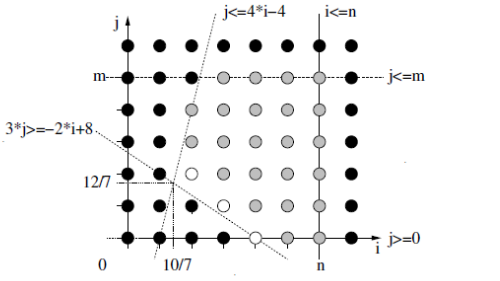
\includegraphics[width=\columnwidth]{poly.png}
	\caption{Representación poliédrica de dos bucles anidados}
	\label{fig:polytope_1}
\end{figure}
%%%%%%%%%%%%%%%%%%%%%%%%%%%%%%%%%%%%%%%%%%%%%%%%%%%%%%%%%%%%%%%%%%%%%%%%%%%%%%%%%%%%%%%%%%

La Matriz \ref{ec:matrix_1} que representa las restricciones de la serie de bucles 
anidados en el Listado \ref{code:polycode1}, delimitará el espacio de iteraciones descrito 
mediante un polígono regular. 
Al tratarse en este caso de un polígono de dos dimensiones se trata de un poliedro, pero 
en general, para espacios de iteraciones $n$-dimensionales, cuando existen $n$ 
bucles anidados, se habla del concepto topológico de politopo.

\subsection{Transformación afín}

%
% ---------------------------------------------------
%
% Proyecto de Final de Carrera:
% Author: José Lucas Grillo Lorenzo <jlucas.gl@gmail.com>
% Capítulo: Yet Another Compiler Framework
% Fichero: Cap4_YaCF.tex
%
% ----------------------------------------------------
%

\cleardoublepage

\chapter{Yet Another Compiler Framework}
\label{chap:yacf}  

%%%%%%%%%%%%%%%%%%%%%%%%%%%%%%%%%%%%% Note %%%%%%%%%%%%%%%%%%%%%%%%%%%%%%%%%%%%%%%%%%%%%
% \begin{mdframed}[backgroundcolor=lightlightgray]
% \textbf{Nota de reconocimiento}
% 
% \small
% Por su relevancia en este \ac{PFC}, enmarcado en el desarrollo llevado a cabo por 
% el equipo de desarrolladores de \accULL{}, se incluye en esta memoria el presente cápitulo,
% extraido y traducido por el autor, a partir del trabajo realizado por \codirectorthesis{},
% \directorthesis{} y su equipo en el TechReport \ref{}. XXX referencia al TechReport de yacf
% \end{mdframed}
%%%%%%%%%%%%%%%%%%%%%%%%%%%%%%%%%%%%%%%%%%%%%%%%%%%%%%%%%%%%%%%%%%%%%%%%%%%%%%%%%%%%%%%%
% \vspace{0.5cm}

\noindent
\acf{yacf} es un compilador \sts{} escrito en Python que ha sido diseñado para facilitar 
el trabajo a los diseñadores de compiladores.
Está dividido en componentes independientes y puede emplearse en desarrollar drivers
\ac{StS} o en crear pequeñas transformaciones de prueba.
Dentro de \yacf{} existen tres paquetes estructurados en módulos y subclases que
resuelven algunos problemas comunes en la traducción de código \ac{StS}.


%%%%%%%%%%%%%%%%%%%%%%%%%%%%%%%%%%%%% Table %%%%%%%%%%%%%%%%%%%%%%%%%%%%%%%%%%%%%%%%%%%%%
\begin{table}[htpb]
\centering
\begin{tabular}{ | l | c | }
  \hline
  \textbf{Parámetro} & \textbf{Valor}                        \\ \hline
  \texttt{loop\_variable} & $i$                                        \\ \hline
  \texttt{\_stride} & $1$                                               \\ \hline
  \texttt{cond\_node} & $i < N$                               \\ \hline
  \texttt{last\_iteration} ($It_{last}$) &  $N-1$  \\   \hline
  \texttt{number\_of\_iterations} & $ ( It_{last} - It_{first} ) / 1 $  \\ \hline
  \texttt{iteration\_expression} & $i += 1$                                        \\  \hline
\end{tabular}
\caption{Información extraída del bucle del Listado \ref{middle:analysis1}}
\label{middle:analysis2}
\end{table}
%%%%%%%%%%%%%%%%%%%%%%%%%%%%%%%%%%%%%%%%%%%%%%%%%%%%%%%%%%%%%%%%%%%%%%%%%%%%%%%%%%%%%%%%%

\lstinputlisting[float,language=C,caption={Un bucle C canónico},label={middle:analysis1}]{listings/analysis1.c} %% LISTING

Nótese que algunos de los parámetros obtenidos no son valores constantes, sino expresiones en lenguaje \ac{IR}.
Estas expresiones serán luego traducidas al lenguaje original por una clase \ac{writer}.
El valor final será evaluado en tiempo de ejecución.

%%%%%%%%%%%%%%%%%%%%%%%%%%%%%%%%%%%%%%%%
\subsection{Optimizaciones de bucles}
\label{subsec:loopopt}

%The optimization stage is one of the most important in any compiler.
%Its function is to improve the performance of object code execution.
%The compilers can optimize the code to improve instructions scheduling, 
%the use of records, or to expose parallelism.
%\cite{Xue:2000:LTP}. % Pag. 43-45
\noindent
Debido a la naturaleza de los compiladores \ac{StS}, las optimizaciones de bucles juegan un papel dominante en 
las optimizaciones de código. \yacf{} implementa varias optimizaciones de bucles como \texttt{interchange}, 
\texttt{unswitch}, \texttt{unroll}, o \tiling{}, algunas de las cuales se describen en detalle a continuación.
Estas transformaciones aparecer con diferentes nombres en la literatura relacionada,
y muchas de ellas han sido implementadas en otros compiladores \ac{StS} tales como Cetus 
\cite{Lee:2003:CEC} o Mercurium \cite{URL::Mercurium}.

Las optimizaciones disponible en \yacf{} han sido implementadas siguiendo
los patrones de software \class{Mutator} y \class{Visitor} \cite{Gamma:1994:DPE}
en el directorio \directory{MiddleEnd.Loop.Mutator}.
Este directorio contiene los mutadores responsables de llevar a cabo el procesamiento sobre el
código intermedio IR-2 (Sección \ref{subsec:IR}).
Por ejemplo, el módulo \module{LoopTiling.py} contiene la clase \class{LoopTilingMutator}
que se encarga de aplicar un \tiling{} rectangular sobre el \ac{AST} suministrado,
p.e. un \tiling{} con tamaños de bloque constante (véase la Sección \ref{LoopTilingRectangular} para más detalles).

Estos mutadores hacen uso extensivo de las herramientas que proporciona el framework \yacf{} como 
\class{ParametrizeLoopTool} para gestionar los bucles, o las disponibles en el paquete 
\package{Tools.Tree} como por ejemplo \class{ReplaceTool}.

En \yacf{} el programador es responsable de verificar la legalidad de las optimizaciones 
que desee aplicar.
Esto es, no hay garantía de que después de aplicar algunas transformaciones tales como 
\tiling{},
la semántica original del código fuente se conserve.
Es responsabilidad del usuario de \yacf{} asegurar la fidelidad al original del programa
optimizado.
%%%%%%%%%%%%%%%%%%%%%%%%%%%%%%%%%%%%%%%%
\subsubsection{El paquete común para optimizaciones de bucles	}
\noindent
El paquete \package{Common.py} del directorio \directory{MiddleEnd.Loop} contiene
varias clases \class{Mutators} y \class{Filters} comunes a muchas optimizaciones y drivers, como
el filtro \class{LoopFilter}.
Este \class{Filter} busca un nodo \class{For} en todo el \ac{AST}.

El comportamiento por defecto de \class{LoopFilter} es iterar sobre el \ac{AST} para devolver
cada uno de los nodos \class{For} encontrados.
A su vez, este filtro puede ser parametrizado con un \textit{identificador} que 
discrimine por la variable índice del bucle, indicándole el bucle o bucles que se desea encontrar.
%%%%%%%%%%%%%%%%%%%%%%%%%%%%%%%%%%%%%%%%
\subsubsection{Loop Interchange}
\label{subsec:interchange}

\noindent
Esta transformación modifica el orden de bucles, intercambiando dos bucles perfectamente anidados.
Uno de los objetivos del \textit{loop interchange} es mejorar el rendimiento de la cache al acceder a
elementos de un array.
Intercambiar los índices de los bucles no siempre es legal debido a las posibles dependencias existentes
entre sentencias y el orden en el que se deben ejecutar. 
Para determinar si un compilador puede intercambiar legalmente dos bucles se debe realizar primero un 
análisis de dependencias entre iteraciones.

\lstinputlisting[float,language=C,caption={Bucle anidado antes de aplicar \textit{loop interchange}},label={code:interchange1}]{listings/interchange1.c} %% LISTING

En el ejemplo básico mostrado en los Listados \ref{code:interchange1} y \ref{code:interchange2}
se puede observar el efecto de la transformación.

\lstinputlisting[float,language=C,caption={Resultado de aplicar \textit{loop interchange} a los bucles anidados del Listado \ref{code:interchange1}},label={code:interchange2}]{listings/interchange2.c} %%<----LISTING


%%
% ---------------------------------------------------
%
% Proyecto de Final de Carrera:
% Author: José Lucas Grillo Lorenzo <jlucas.gl@gmail.com>
% Capítulo: Optimizaciones en GPGPU
% Fichero: Cap5_Opt_GPGPU.tex
%
% ----------------------------------------------------
%

\chapter{Optimizaciones en \gpgpu{}}
\label{chap:optGPGPU}

En este Capítulo se pone de manifiesto la investigación en optimizaciones para
arquitecturas \gpgpu{} usando
el compilador \yacf{}. Una herramienta de compilación \ac{StS} con la 
que el autor ha podido desarrollar algunas técnicas de optimización bien conocidas para 
\gpgpu{} en el marco de la versión 1.0 del estándar \ac{OpenACC}.

% Ecribir sobre \gpgpu{} y el \tiling{} para \gpgpu{}

\section{Arquitecturas \gpu{}s}
\label{sec:arquitecturasGPU}

% Concepto de kernel 
Las \gpu{}s son arquitecturas que explotan el paralelismo a nivel de \thread{}s. En este 
contexto se define un \thread{}, o hilo, como un conjunto de instrucciones simples que han 
de ser ejecutadas de forma independiente y paralela. Estas instrucciones simples están 
definidas en lo que se conoce como \textit{kernel}, que no es más que un código fuente, 
generalmente escrito en un subconjunto de C con extensiones para ser ejecutado por un 
conjunto de \thread{}s en un dispositivo acelerador.

Estos conceptos son habituales para un programador de \CUDA{} y también extensibles a 
\OpenCL{}. Por simplicidad, se tratan ahora algunos aspectos de la arquitectura \CUDA{}. 
La arquitectura de \OpenCL{} es ligeramente distinta pero no se entrarán en esos detalles
diferenciadores al no resultar relevantes.

\subsection{Modelos arquitecturales lógico y hardware: CUDA}

% Describir modelo lógico(CUDA) y hardware
% Añadir imagenes de la arquitectura CUDA
% Describir mínimamente la jerarquía de threads
%%%%%%%%%%%%%%%%%%%%%%%%%%%%%%%%%%%%% Figure %%%%%%%%%%%%%%%%%%%%%%%%%%%%%%%%%%%%%%%%%%%%%
\begin{figure}[!h]
	\centering
	\includegraphics[width=0.8\linewidth]{CUDA_logical.png}
	\caption{Modelo lógico de \CUDA{}}
	\label{fig:CUDAlogical}
\end{figure}
%%%%%%%%%%%%%%%%%%%%%%%%%%%%%%%%%%%%%%%%%%%%%%%%%%%%%%%%%%%%%%%%%%%%%%%%%%%%%%%%%%%%%%%%%%

El modelo teórico de \CUDA{} representado en la Figura \ref{fig:CUDAlogical} asume que se 
dispone de un número infinito de \thread{}s en 
ejecución, pero no garantiza que esos \thread{}s estén ejecutándose a la vez. Si la 
pregunta es cuantos \thread{}s se ejecutarán simultáneamente, la respuesta será que 
esto depende de la arquitectura hardware, no de la lógica. Como el hardware cambia con 
rapidez, la arquitectura lógica intenta simplificar esto
permitiendo a los usuarios definir una partición lógica de \thread{}s y bloques de 
\thread{}s. De esta forma, los \thread{}s dentro de un bloque se ejecutarán 
simultáneamente, mientras que los bloques de \thread{}s pueden ejecutarse a la vez o no,
según lo recursos hardware disponibles. El conjunto de bloques de \thread{}s es lo que se 
denomina \textit{grid}.

%%%%%%%%%%%%%%%%%%%%%%%%%%%%%%%%%%%%% Figure %%%%%%%%%%%%%%%%%%%%%%%%%%%%%%%%%%%%%%%%%%%%%
\begin{figure}[!h]
	\centering
	\includegraphics[width=0.8\linewidth]{SMFermi.png}
	\caption{Diagrama de un \textit{Streaming Multiprocessor} de la arquitectura Fermi de \NVIDIA{}}
	\label{fig:SMFermi}
\end{figure}
%%%%%%%%%%%%%%%%%%%%%%%%%%%%%%%%%%%%%%%%%%%%%%%%%%%%%%%%%%%%%%%%%%%%%%%%%%%%%%%%%%%%%%%%%%

% Describir mínimamente los warps
La unidad mínima de un bloque de \thread{}s, en la arquitectura CUDA, es lo que de conoce 
como \warp{}. Equivale a 32 threads, aunque este número pudiera cambiar en un futuro. Los 
\ac{SM} como el mostrado en la Figura \ref{fig:SMFermi}, crean, gestionan, planifican
y ejecutan los \thread{}s con granularidad de \warp{}, de tal forma que todos los 
\thread{}s de un \warp{} ejecutan la misma instrucción a la vez. Aunque en el caso de que 
aparezcan divergencias condicionales, el \warp{} ejecuta secuencialmente cada una de las 
ramas tomadas.

%Cuando se accede a la memoria global, se trata de que los accesos de los \thread{}s de un 
%warp sean coalescentes, empleando el menor número de transacciones posibles.

\section{El estándar \ac{OpenACC}}

% El modelo de programación para arquitecturas heterogeneas basado en directivas
% Introducción *muy básica* al estándar y descripción mínima de su uso

% Ecribir introducción básica sobre \ac{OpenACC}
El estándar \OpenACC{} v1.0 \cite{URL::OpenACC} define un modelo de programación para 
arquitecturas heterogéneas basado en directivas.
Fue publicado en noviembre de 2011 y ha servido para apoyar todo el 
desarrollo que se venía realizando el grupo \GCAP{} en este campo.

En la primera versión de dicho estándar, se introducen directivas y cláusulas para la 
gestión de códigos orientados a ser 
ejecutados en las \gpu{}s. Así como la gestión de las transferencias de memoria entre 
CPU (\textit{host}) y \gpu{} (dispositivo acelerador),
críticas para una buena implementación en este tipo de arquitecturas.

Como ejemplos de dichas directivas, el estándar introduce \texttt{\#pragma acc data}, que 
mediante cláusulas como \texttt{copyin} o \texttt{copyout}, permite indicar al 
compilador que una lista de variables debe ser transferida respectivamente hacia o desde 
el dispositivo.

En la versión 1.0 de \OpenACC{}, las directivas encargadas de extraer un código a la 
\gpu{} son: \texttt{\#pragma acc kernels} que indica que la siguiente región de código
ha de generar uno o varios kernels en función de los bucles encontrados en dicha región;
y \texttt{\#pragma acc parallel} que indica que la región de código ha de ejecutarse en un
único kernel. 

La directiva \texttt{kernels} no tiene sentido sin marcar los bucles que
deben ser analizados. Para ello, se emplea la cláusula \texttt{loop} que etiqueta el bucle
inmediatamente a continuación de la \texttt{\#pragma} que contiene dicha cláusula.

Por otra parte, y aunque la directiva \texttt{parallel} no depende necesariamente de la 
existencia de bucles en su región, sí es posible etiquetar los bucles dentro de una región 
\texttt{parallel} para indicar así que el espacio de iteraciones de estos bucles debe
ser distribuido entre los \thread{}s disponibles.


\subsection{Sobre gangs y workers en \ac{OpenACC} v1.0}
\label{subsec:gangsworkers}
% Introducir correlación entre gangs/workers y thread-blocks/threads.
% Añadir \ref{sec:arquitecturasGPU}
Como se describe en la Sección \ref{sec:arquitecturasGPU}, en las arquitecturas \gpu{} 
las unidades de cómputo se estructuran en bloques de \thread{}s
de tamaño determinado, y agrupaciones independientes de bloques de \thread{}s en 
\grid{}s.

% Meter la gráfica donde se ve la *fuerte* dependencia de los compiladores actuales de los 
% valores de gang-worker
% Cita al estándar donde se describen gang y worker
El estándar \ac{OpenACC} \cite{URL::OpenACC} introdujo las 
cláusulas \gang{}, \worker{} y \cvector{} para las regiones \texttt{kernels}, y
\texttt{num\_gangs} , \texttt{num\_workers} y \texttt{num\_vectors} para las regiones \texttt{parallel}.
Estas cláusulas tienen como principal objetivo 
dar al programador mayor control sobre la planificación del código que 
se descarga al acelerador.

Aunque el estándar no determina detalles de su implementación,
en el desarrollo de los compiladores recientes en los que se ha abordado la integración de 
\ac{OpenACC}, se han tomado distintas soluciones para las cláusulas que nos ocupan. En 
algunas implementaciones como las seguida por \CAPS{} y la descrita aquí para 
\accULL{}, se ha optado por dar uso a solo dos de estos niveles: \textit{gang}s, 
correspondiente a grupos de bloques; y \textit{worker}s, para determinar el tamaño de 
los bloques de {thread}s. Reservando la cláusula \cvector{} para una futura aplicación
a instrucciones vectoriales \SIMD{} dentro de cada \thread{}.
% jerarquía de \thread{}s, por \grid{} y por bloques de \thread{}s,

Las cláusulas \texttt{num\_Xs} fijan un tamaño de cada nivel de planificación \texttt{X}, 
para las regiones \texttt{parallel} que las contienen. Así, los tamaños de 
\textit{worker}s y \textit{gang}s asignados respectivamente 
a una serie de bucles etiquetados con la cláusula \texttt{loop}, determinarán las 
dimensiones de esta asignación jerárquica de \thread{}s. Es decir, por ejemplo, las 
iteraciones de un bucle etiquetado con \texttt{\#pragma acc loop gang(64) worker(32)} o
una región \texttt{\#pragma acc parallel loop num\_gangs(64) num\_workers(32)},
distribuirán las iteraciones del bucle entre \texttt{64} bloques de \thread{}s, con 
\texttt{32} \thread{}s cada bloque.
% Cláusulas con tamaño fijo vs cláusulas sin tamaño explícito: que el compilador lo determine
También es posible no indicar explícitamente el tamaño de la distribución jerárquica de
threads, dejando así que el compilador la decida.

En definitiva, las cláusulas \gang{}, \worker{} y \cvector{} pueden ayudar al compilador a 
mapear el espacio de iteraciones de los bucles a la arquitectura subyacente.

\subsection{\tiling{} para mapear un espacio de iteraciones}
\label{subsec:tmaping}
% Estructura por bloques de threads y grids de bloques en \gpgpu{}: Su interpretación en 
% las cláusulas
La interpretación de las cláusulas, citadas en la Sección anterior, seguida en \accULL{} 
ha sido una implementación por \textit{tiles}, o bloques de iteraciones. 
Empleando la transformación \tiling{} descrita en la Sección \ref{subsec:LoopTiling},
también conocida como \textit{blocking} multidimensional.

Esta es una optimización bien conocida desde hace varias décadas 
\cite{Wolfe:1987:IST,Wolfe:1989:MIS},
y recientemente ha resurgido como método para mejorar las prestaciones de códigos \CUDA{} 
\cite{BON:ATC:2008} y en general para dispositivo aceleradores.

%Entre otras utilidades, puede aprovecharse para explotar los múltiples niveles 
%jerarquicos de memoria en arquitecturas como las \gpu{}s. Esto se logra reasignando el 
%espacio de iteraciones a las unidades de cómputo (PEs) siguiendo un esquema jeráquico.

% ¿ Porqué usar \tiling{} con estas cláusulas ?
La estrategia adoptada por el compilador de \CAPS{} para \OpenACC{} en la implementación 
de las cláusulas, ha consistido en seguir una variante del \tiling{} en la que se segmenta 
el espacio de iteraciones en bloques de iteraciones, que se asignan en \gpu{} 
a un número determinado de bloques de \thread{}s (número de \gang{}s) y a un número 
determinado de \thread{}s por cada bloque de \thread{}s (número de \worker{}s).
Por último cada \thread{} recorre su \textit{tile}, de iteración en iteración, 
para respetar el espacio de iteraciones original.

En \accULL{} se decidió adoptar una estrategia similar, siguiendo el modelo clásico de 
\tiling{} asignando \textit{tile}s a \thread{}s como se ha descrito. 
%%% TODO: Como de similar: Strip2Mutator (CAPS o PGI)?? por StripMiningMutator (accULL)
En el caso del compilador de PGI para \OpenACC{} la estrategia difiere, ya que considera 
que los \textit{woker}s han de mapeares con los \warp{}s descritos en la Sección 
\ref{sec:arquitecturasGPU}, mientras que es la cláusula \cvector{} es la que mapea a 
\thread{}s. Dejando al usuario programador la elección de \gang{}s y \cvector{} en lugar 
de \gang{}s y \worker{}s implementada por \CAPS{} y \accULL{}.
%En el caso de CAPS y \accULL{}, se reserva la cláusula \texttt{vector} para una 
%implementación de instrucciones vectoriales SIMD, tal como sugiere el estándar
%de OpenACC \ref{URL::OpenACC}.

%%%%%%%%%%%%%%%%%%%%%%%%%%%%%%%%%%%%% Figure %%%%%%%%%%%%%%%%%%%%%%%%%%%%%%%%%%%%%%%%%%%%%
\begin{figure}[h]
   \centering
   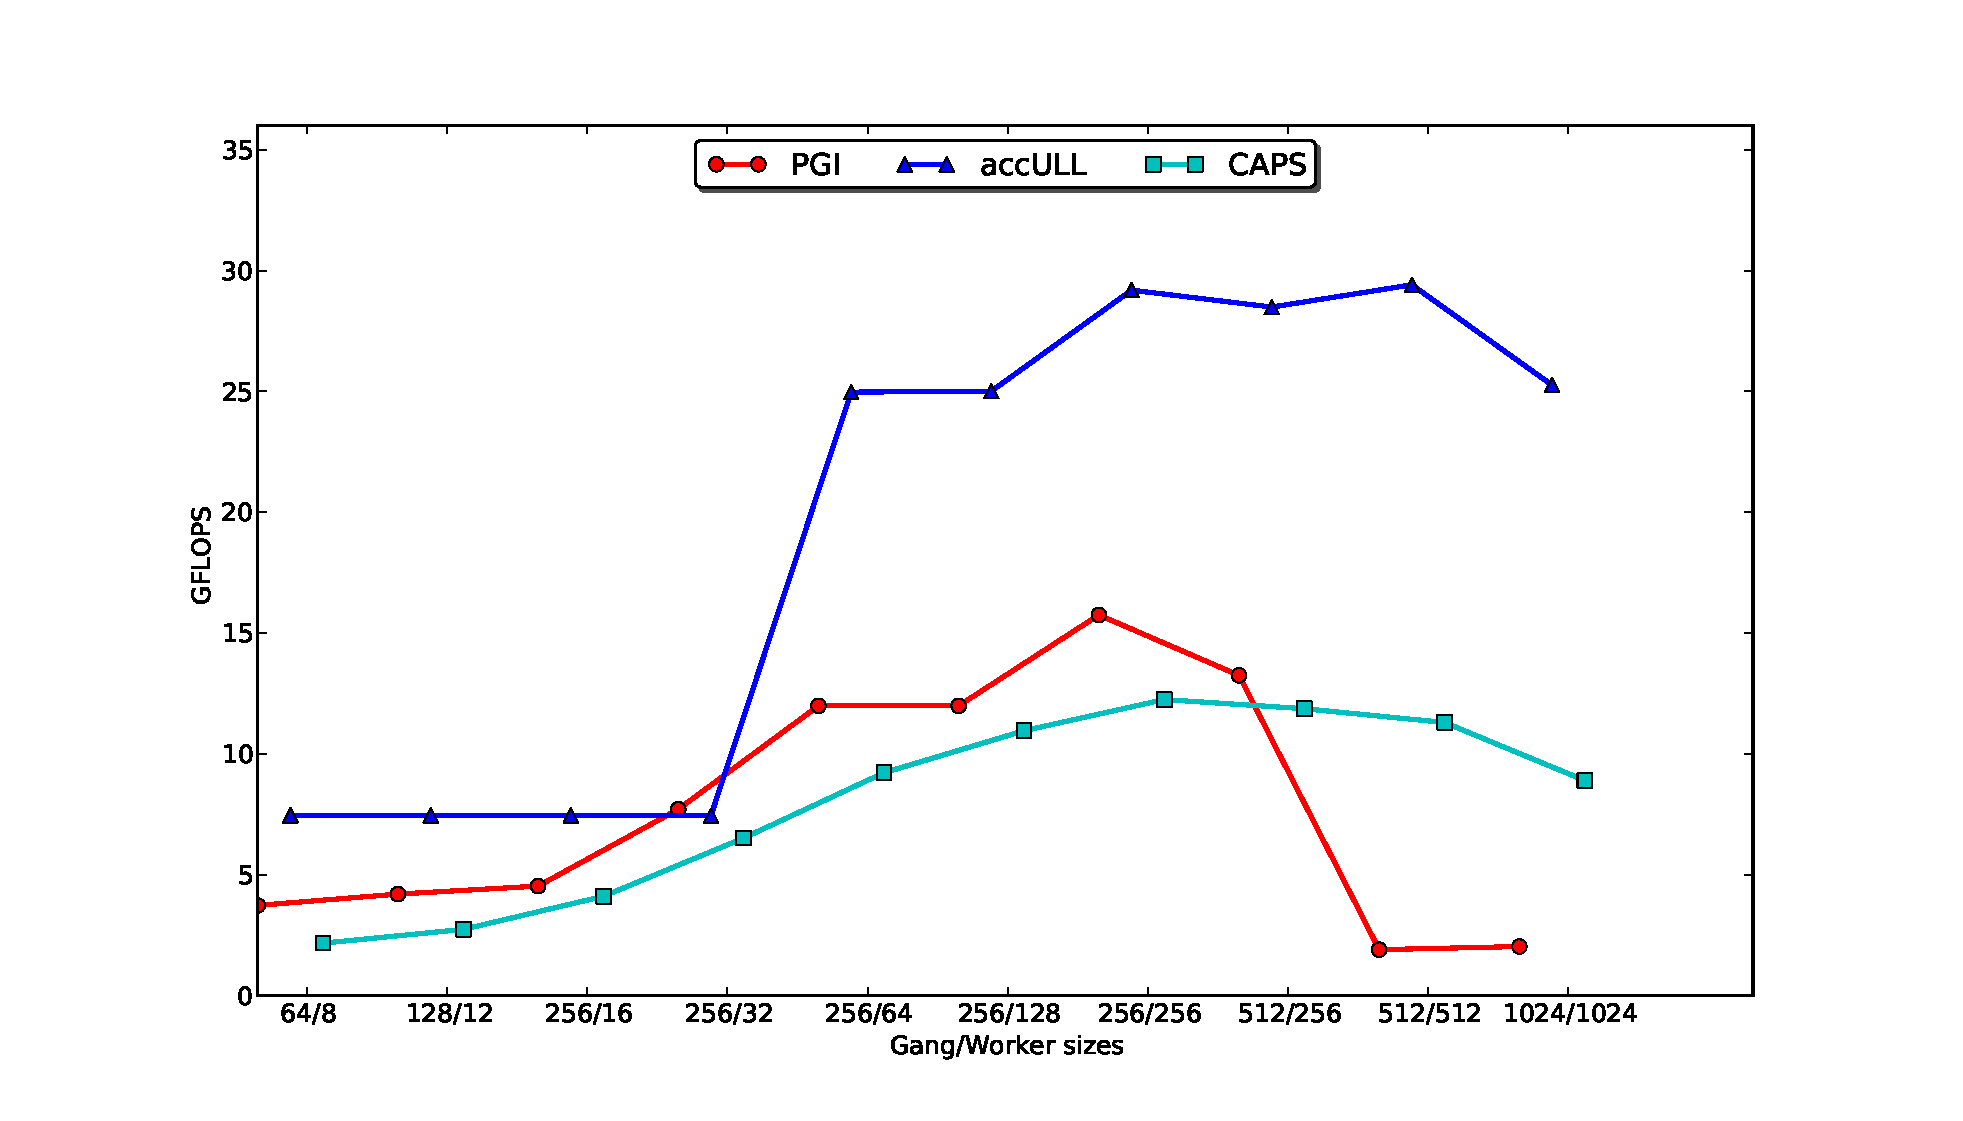
\includegraphics[width=\textwidth]{FIGURES/gemm_flops_varying}
   \caption{Rendimiento de un código evaluado con distintos valores \gang{}/\worker{} para un mismo entorno de ejecución.}
   \label{fig:gemm_gangworker_1}
\end{figure}
%%%%%%%%%%%%%%%%%%%%%%%%%%%%%%%%%%%%%%%%%%%%%%%%%%%%%%%%%%%%%%%%%%%%%%%%%%%%%%%%%%%%%%%%%%

% Revisar resultados del MxM
Los resultados obtenidos en la comparativa de la Figura \ref{fig:gemm_gangworker_1} 
nos hacen pensar que esta interpretación es buena, y puede llegar tomarse como modelo a 
seguir por otros proyectos similares. Se puede deducir una fuerte dependencia de la 
implementación elegida, en la notable 
diferencia entre los resultados mostrados en la Figura \ref{fig:gemm_gangworker_1} al 
ejecutarse un código de multiplicación de matrices etiquetado con \ac{OpenACC} con 
varios compiladores con soporte \OpenACC{} y varios tamaños de \gang{} y \worker{}, o 
\gang{} y \cvector{}.

% Automatizar la generación de una implementación por bloques mediante las cláusulas gang 
% y worker
A continuación se describe el procedimiento seguido para automatizar esta interpretación 
del estándar por bloques.

\section{Mutadores de \yacf{} implicados en la transformación}
\label{sec:mutatorstiling}
%XXX Escribir introducción. Nombrar ASTs y mutadores. Uso amplio de las herramientas 
%desarrolladas en \yacf{}.

Las transformaciones de código intermedio (ver Sección \ref{subsec:IR}) se pueden 
lograr aplicando mutadores (ver Sección \ref{subsec:mutator}) y filtros (ver Sección 
\ref{subsub:filter}) que seleccionen los segmentos del \ac{AST} que ha de ser 
transformado. En este trabajo se ha hecho uso amplio de las herramientas desarrolladas
en \yacf{} como se ha mencionado en la Sección \ref{subsec:loopopt}.

%XXX Escribir sobre el mutador \package{LoopTilingMutator} y su descomposición en los 
%mutadores \package{LoopStripMining} y \package{LoopInterchangeMutator}.

En la Sección \ref{subsec:LoopTiling} se describe en detalle como se descompone el mutador 
\package{LoopTilingMutator} en los mutadores \package{LoopStripMining} y 
\package{LoopInterchangeMutator}, donde se incluye el algoritmo seguido
para este fin (Algoritmo \ref{alg:tiling}).


\subsection{El módulo \package{LoopInterchangeMutator.py}}
Inicialmente este módulo estaba definido como un
intercambiador de dos bucles perfectamente anidados consecutivos, y atendía a las 
cláusulas \llc{} \cite{URL::LLC} heredadas de la investigación llevada a cabo por el grupo
\cite{Garcia:1997:LLC,Luna:1998:HED} \cite{Almeida:2003:PSU,Dorta:2003:LPS}
\cite{Reyes:2011:ACG}. 

Para emplearse y ser realmente útil en la implementación
seguida del \package{LoopTilingMutator} fue necesario remodelarlo completamente. Aunque ha 
quedado en desuso, se ha mantenido la retrocompatibilidad con las cláusulas \llc{} 
originales.

A continuación se detallan los requisitos de este mutador  de cara a la implementación del 
driver descrito en la Sección \ref{chap:optGPGPU:accgangworker}:

\begin{itemize}
\item Dar múltiples opciones al desarrollador de drivers para un uso versátil del mutador 
en el paso de parámetros y establecer un comportamiento por defecto basado en el mutador 
original.
\item Permitir intercambiar dos bucles cualesquiera en un anidamiento perfecto, 
indistintamente de su nivel de profundidad o del orden en el que se le indicase (más 
profundo por menos profundo o viceversa).
\item Asociar a cada bucle las posibles directivas que etiquetasen el bucle.
\end{itemize}

El comportamiento por defecto indicado en el primer punto es el intercambio de los dos 
bucles anidados inmediatamente siguientes al AST suministrado, que es el único parámetro 
requerido en todo mutador. El intercambio flexible de bucles era necesario para su 
integración en el \package{LoopTilingMutator}, ya que es parte del Algoritmo 
\ref{alg:tiling} descrito en la Sección \ref{subsec:LoopTiling}. Por último, era vital
asociar a los bucles intercambiados las posibles pragmas para conservar su significado 
original en el código resultante. Con esto se pretende que las directivas queden en los 
bucles externos al aplicar \tiling{}, y así se puedan paralelizar éstos, enviando a \gpu{} 
los bucles internos. 

%Describir minimamente implementación en cuatro pasos del mutador
El comportamiento de este mutador se describe en detalle en la Sección 
\ref{subsec:interchange}.
%La implementación en cuatro pasos del mutador ... 

\subsection{El módulo \package{LoopStripMiningMutator.py}}

Inicialmente este módulo era la implementación original del \tiling{}. En los ejercicios 
iniciales, la transformación se aplicaba a bucles individuales y no había reordenación, 
con la consecuente falta de coherencia en el resultados del código final.

En la práctica, como se indica en la Sección \ref{subsec:Strip-mining}, aplicar \tiling{} a un único 
bucle es equivalente a aplicar a dicho bucle \textit{Loop Strip-Mining}.
De esta manera, siguiendo nuestra metodología de desarrollo continuo, hemos generalizado 
el código que se describe a continuación:

\begin{itemize}
\item Obtener los parámetros y variables necesarias a partir del \ac{AST} suministrado
\item Generar un nuevo bucle con una nueva variable índice que itere sobre los bloques 
\item Modificar el bucle original para que itere dentro de cada bloque
\item Sustituir el nuevo \ac{AST} por el \ac{AST} original y generar las declaraciones 
necesarias y situarlas justo antes del bucle más externo en el orden adecuado
\end{itemize}

El comportamiento de este mutador se describe en detalle en la Sección \ref{subsec:Strip-mining}. Un ejemplo del resultado de este mutador se puede observar en el Listado \ref{code:looptilingmutator1}
después de aplicarlo al código del Listado \ref{code:looptilingmutator0}. 

\subsection{El módulo \package{LoopTilingMutator.py}}
\label{subsubsec:looptilingmutator}

% Escribir detalles de implementación del Algoritmo \ref{alg:tiling}

Es importante destacar que en la implementación del \package{LoopTilingMutator.py} se ha 
optado por dividir el número de iteraciones de los bucles originales por el número de 
\gang{}s y/o \worker{}s, tal y como se describe en la Sección \ref{subsec:gangsworkers},
asignando el código resultante al tamaño del \textit{tile}, y consiguiendo dividir el 
espacio de iteraciones en el número de \gang{}s y \worker{}s solicitado.

\lstinputlisting[float,language=C,caption={Bucle de 10 iteraciones que asigna el número de 
iteración a un vector del mismo tamaño}, label={code:looptilingmutator0}]
{listings/looptilingmutator0.c} %% LISTING

En el Listado \ref{code:looptilingmutator1} se puede observar como la variable 
\texttt{remain\_i} (línea 4) es la que contiene dicho resultado. En la línea 9 se calcula 
la última iteración del bucle interno, garantizando que no se supera el tamaño original.
El Algoritmo \ref{alg:tiling} y la implementación seguida para este módulo se describe en 
detalle en la Sección \ref{subsec:LoopTiling}.

\lstinputlisting[float,language=C,caption={Código resultante de la aplicación del mutador \package{LoopTilingMutator.py}
al código del Listado \ref{code:looptilingmutator0}},
label={code:looptilingmutator1}]{listings/looptilingmutator1.c} %% LISTING


\subsection{Acerca del \driver{} \textit{accgangworker.py}}
\label{chap:optGPGPU:accgangworker}

%XXX Ecribir descripción

% Descripción del driver accgangworker.py
% Sigue el patrón de drivers desarrollados para yacf
% Pasos de la transformación StS: 
%       FrontEnd ( parseo ), anotación de la IR, ...
%                aplicación de la tranformación a las cláusulas
%                generación de código final ( C + OpenACC )

En el transcurso del trabajo realizado se ha desarrollado un \driver{} siguiendo el 
esquema definido en la Sección \ref{chap:yacf:design}, para el análisis y la verificación 
de la correcta implementación de la transformación seguida para las cláusulas \gang{} y 
\worker{}.

Este \driver{} sigue el modelo de ejecutables definido para \yacf{}. Con un análisis 
inicial en el \package{frontend} \ref{subsec:Frontend}, seguido de las correspondientes 
anotaciones de la \ac{IR} \ref{subsec:IR}, la aplicación de los filtros y mutadores, y por 
último un volcado del código resultante mediante el \writer{} %\ref{subsec:writer}
de \OpenACC{} \ref{subsect:AccWriter}.

La estrategia seguida para aplicar \tiling{} a las cláusulas \gang{} y \worker{} ha sido 
filtrar primero todas las cláusulas \worker{}, aplicar \tiling{}. Por último se filtran 
las cláusulas \worker{} y se aplica el mutador de nuevo.

De esta manera, se consigue segmentar el espacio de iteraciones en cada bloque de threads,
inicialmente usando el número de \worker{}, y posteriormente repitiendo el proceso para 
todo el \grid{}, aplicando la planificación de los \gang{}.

\section{Las regiones \texttt{parallel}}

En la versión 0.3 de \accULL{} se ha añadido soporte para los bucles que se encuentran 
dentro de las regiones \texttt{parallel} - que hasta ahora eran ejecutados 
secuencialmente. 
Para ello se ha implementado un mutador (\class{AccParallelLoopMutator}) que genera código 
capaz de 
distribuir las iteraciones de los bucles entre los \thread{}s/bloques que conforman el 
grid en ejecución. Dicho mutador resuelve la distribución de los bucles anidados mediante 
recursividad. 

\lstinputlisting[float,language=Python,caption={Mutador recursivo AccParallelLoop 
utilizado para la paralelización de las iteraciones dentro de cláusulas 
\texttt{parallel}}, label={code:accparallelloop}]
{listings/accparallelloop.py} %% LISTING

El Listado \ref{code:accparallelloop} muestra una versión simplificada de la 
implementación del mutador. Como se puede observar, en la línea 6 se filtra el \ac{AST}
suministrado buscando la cláusula \texttt{loop}. Una vez obtenida, se extrae el bucle
asociado (línea 8) y éste se parametriza en el diccionario \texttt{loop\_parameters} 
(línea 18). El código interno del bucle se asigna al parámetro \texttt{'code'} dentro del 
diccionario \texttt{system\_parameter}. Ambos diccionarios son aplicados a la plantilla
mostrada en el Listado \ref{code:template_ploop} como \texttt{'l\_p'} y \texttt{'s\_p'} respectivamente, que 
posteriormente es parseada mediante la función heredada \texttt{parse\_snippet} (línea 
25). En la línea 30 se aplica la herramienta \class{ReplaceTool} descrita en la Sección
\ref{subsec:handleIR}, para retirar del \ac{AST} las directivas asociadas al bucle.

Finalmente en la línea 34 se hace una llamada recursiva al mutador. Las líneas 11, 14-15 y 
38 controlan la recursividad del mutador, no permitiendo más de dos niveles de 
anidamiento. Además en ningún momento se aplicarán más niveles de recursividad que bucles
anidados estén etiquetados. Esto se controla al disparar una excepción de tipo 
\texttt{NodeNotFound} cuando no se ha encontrado una cláusula \texttt{loop}, rompiendo así
la recursividad.

\lstinputlisting[float,language=C,caption={Plantilla para el mutador recursivo mostrado en
el Listado \ref{code:accparallelloop}}, label={code:template_ploop}]
{listings/template_ploop.c} %% LISTING

\subsection{Ecuaciones de distribución de iteraciones}
\label{subsec:ecuations}

\lstinputlisting[float,language=C,caption={Bucle etiquetado con la cláusula \texttt{loop} 
dentro de una región \texttt{parallel}}, label={code:ploop}]
{listings/parallel_loop.c} %% LISTING

\lstinputlisting[float,language=C,caption={Código del kernel correspondiente al bucle 
etiquetado en el Listado \ref{code:ploop}, después de aplicar el mutador mostrado en
el Listado \ref{code:accparallelloop}}, label={code:ploop_mutated}]
{listings/parallel_loop.cu} %% LISTING


%Cláusulas numgang y numworker en \ac{OpenACC} v1.0
La plantilla mostrada en el Listado \ref{code:template_ploop} genera una serie de 
ecuaciones en lenguaje C destinadas a distribuir las iteraciones de un bucle entre 
\thread{}s y bloques de \thread{}s tal y como se explicó en la Sección 
\ref{subsec:tmaping}. El mutador recursivo mostrado en el Listado 
\ref{code:accparallelloop} se encarga de transformar un código como el mostrado en
el Listado \ref{code:ploop} a un código interpretable por el kernel como el que se
muestra en el Listado \ref{code:ploop_mutated}.
En las líneas 2-3 del Listado \ref{code:ploop_mutated} se calcula un tamaño de salto 
(\textit{stride}) para las iteraciones entre bloques (\textit{block}s) y dentro de cada 
bloque (\thread{}s). En las líneas 5-6 se calcula el inicio de del \textit{tile}, y el
las líneas 8-9 el final. Las líneas 11-14 del Listado \ref{code:ploop_mutated} recorren el 
tile correspondiente a cada \thread{}.

Cuando aparezcan dos bucles etiquetados con la cláusula \texttt{loop} dentro de una región
\texttt{parallel} se tratará de distribuir las iteraciones en bloques de threads de dos 
dimensiones. La primera dimensión de threads para el primer bucle y la segunda dimensión
para el segundo bucle. Un problema abierto en \accULL{} es contemplar que estas ecuaciones
solo se apliquen cuando el número de iteraciones a distribuir es igual o mayor que el 
número de \thread{}s disponibles en todas las dimensiones aplicables. Actualmente si no 
se da este caso pude suceder que los resultados no sean los esperados al omitir la 
ejecución de algunas iteraciones.

%%
% ---------------------------------------------------
%
% Proyecto de Final de Carrera:
% Author: José Lucas Grillo Lorenzo <jlucas.gl@gmail.com>
% Capítulo: Resultados computacionales 
% Fichero: Cap7_resultados.tex
%
% ----------------------------------------------------
%

\chapter{Resultados computacionales} \label{chap:resultados}  

En este Capítulo se presentan una serie de resultados evaluando
diversos tests compilados con \accULL{}, y algunos de los compiladores comerciales de 
\OpenACC{} disponibles en el mercado. En él se detalla en qué consisten 
dichos tests y la infraestructura hardware sobre la que se han realizado los experimentos,
así como una comparativa del rendimiento alcanzado con los mismos.
Se describirán posteriormente los tests sobre los que se ha trabajado. 
Concretamente, tres experimentos del conjunto de pruebas \rodinia{} 
\cite{URL::Rodinia}, un código de multiplicación de matrices, y el \benchmark{} para 
\OpenACC{} del \epcc{} publicado recientemente 
en su web \cite{URL::ACCepccB}. Aportando medidas de rendimiento en aceleración o tiempo 
de compilación cuando se dispongan.

\section{Plataforma hardware}

A continuación se describe las características de la plataforma hardware sobre la que
han realizado las pruebas de experimentación:

\begin{itemize}
	\item \texttt{Garoe}: Una \textit{Workstation} con un procesador \textbf{Intel Core i7 930} a 2.80 GHz con 1MB de cache L2 y 8MB de cache L3 compartida por los cuatro núcleos. Este computador tiene 4 GB de memoria RAM y dos \GPU{}'s de \NVIDIA{} conectadas a este sistema: una Tesla M2090 con 512 núcleos CUDA y 5GB de memoria (Fermi), y una Tesla K20c
	con 2496 núcleos CUDA y 4GB de memoria (Kepler).
En este servidor se han realizado las pruebas con los \benchmark{}s de \rodinia{}.
	\item \texttt{Verode}: Un \textit{cluster} que contiene procesadores de dos \textit{quad core} \textbf{Intel Xeon E5410} a 2.25GHz, 24GB de memoria y una \GPU{} Fermi C2050 con 4GB de memoria en el nodo \textit{verode16}. El nodo de compilación \textit{verode00} es virtualizado. En \texttt{Verode} se ha evaluado el rendimiento de \accULL{} con la \epcc{} \OpenACC{} \benchmark{} suite.
\end{itemize}

Con la plataforma \texttt{Garoe} se pretende simular un escenario habitual para un 
desarrollador de \OpenACC{}, es decir, un usuario con cierta experiencia 
interesado en mejorar el rendimiento de un código, podría adquirir una \GPU{} e insertarla
en su sobremesa. Es una solución relativamente barata, a cambio de un incremento
considerable en el rendimiento con muy poco esfuerzo de desarrollo.

En el otro extremo se encuentra \texttt{Verode16}, un nodo de un \textit{cluster}
heterogéneo de alto rendimiento. Los \textit{cluster}s heterogéneos son frecuentes
en los centros de supercomputación de hoy en día. Al estar compuestos por 
sistemas multinúcleo y aceleradores gráficos, se facilita el uso de \OpenACC{} en estas 
plataformas. 

\section{Software evaluado}

En los experimentos realizados se han evaluado tres compiladores con soporte para 
\OpenACC{}. Para el conjunto de tests de la suite \epcc{} \OpenACC{} \benchmark{} se han 
empleado los últimos compiladores disponibles hasta la fecha. En el caso de los resultados 
de los tests \rodinia{} medidos en Garoe se incluyen resultados obtenidos con versiones anteriores de los
compiladores por tener una referencia comparativa.
A continuación se muestra una descripción de los compiladores empleados en cada caso:

\begin{itemize}
\item \PGI{} OpenACC en su versión 12.5 para el \benchmark{} \rodinia{} y la multiplicación de matrices (MxM), usando la versión 13.5 (la más reciente hasta la fecha) para la suite \epcc{} \OpenACC{} \benchmark{}. 
\item \CAPS{} HMPP con soporte para \OpenACC{}, versión 3.3.3 para la suite \epcc{} \OpenACC{}, y la versión 3.3.1 para los tests \rodinia{} y MxM. 
\item \accULL{} versión 0.1b para \rodinia{} \benchmark{} suite y MxM, mientras que  para la suite \epcc{} \OpenACC{} \benchmark{} se ha empleado la versión 0.3alpha.
\end{itemize}

\section{Rodinia \benchmark{} suite}

El conjunto de pruebas \rodinia{} \cite{Che:2010:CRB} está compuesto de 
programas de cómputo intensivo diseñados para ser ejecutados en entornos 
masivamente paralelos como los de una \GPU{}, cubriendo un amplio rango de 
aplicaciones.
La suite incluye versiones para la mayoría de los códigos en OpenMP, CUDA y OpenCL,
demostrando la viabilidad de la programación basada en directivas y su facilidad de uso.
En esta Sección se
presenta el rendimiento para tres \benchmark{}s extraídos de la suite. Dichos 
\benchmark{}s han sido anotados con 
\OpenACC{} a partir de la versión \OpenMP{} con relativa facilidad.
En esta contribución se proporcionan los resultados computacionales de tres códigos:
una descomposición LU (\texttt{LUD}),
una herramienta de simulación térmica (\texttt{HS}) y un método de optimización global 
no lineal para alineamientos de secuencias de ADN (\texttt{NW}).
En las Tablas \ref{table:rodinia:fermi} y \ref{table:rodinia:kepler} se muestra una 
comparativa de rendimiento entre dos \GPU{}s con arquitectura Fermi y Kepler 
respectivamente, 
con las implementación \OpenACC{} usando los compiladores de \PGI{}, \CAPS{} y \accULL{}, 
respecto a la implementación con \CUDA{} nativo.

\subsection{HotSpot (\texttt{HS})}

HotSpot (\texttt{HS}) es una herramienta de simulación térmica usada para
estimar la temperatura del procesador basada en un superficie plana y medidas de 
disipación de potencia simuladas.

La implementación de \rodinia{} incluye el kernel 2D de simulación térmica transitoria
de \texttt{HS},
que calcula iterativamente una serie de ecuaciones diferenciales para bloques de 
temperatura. 
Las entradas al programa son la potencia y las temperaturas iniciales. 
Cada celda de salida de la malla representa el valor de temperatura media del área
correspondiente del chip.

%%%%%%%%%%%%%%%%%%%%%%%%%%%%%%%%%%%%%%%%%%%%%%%%%%%%%%%%%%%%%%
\begin{lstlisting}[caption={Bucle principal de \texttt{HS}},label=code:HS]
for (i = 0; i < num_iterations ; i++) { 
    /* Compute current temperatures */
    for (r = 0; r < row; r++) 
      for (c = 0; c < col; c++) 
          ...
    /* Update */
    for (r = 0; r < row; r++) 
      for (c = 0; c < col; c++) 
          ...
  }
\end{lstlisting}
%	%%%%%%%%%%%%%%%%%%%%%%%%%%%%%%%%%%%%%%%%%%%%%%%%%%%%%%%%%%%%%
El Listado \ref{code:HS} muestra una versión resumida de la rutina principal de
 \texttt{HS}. Contiene dos bucles anidados que se ejecutan durante un número determinado 
de iteraciones. El primer bucle computa la temperatura actual de cada posición dentro del 
chip, mientras que el segundo, solo actualiza los datos con la información calculada en la 
iteración actual.

%%%%%%%%%%%%%%%%%%%%%%%%%%%%%%%%%%%%%%%%%%%%%%%%%%%%%%%%%%%%%%
\begin{lstlisting}[caption={Boceto de \texttt{HS} usando \OpenACC{}},label=code:HS:openacc]
void do_iteration(double * temp,...) {
 #pragma acc kernels ....
   { /* Compute current temperatures */
     #pragma acc loop ... 
     for (r = 0; r < row; r++) 
       for (c = 0; c < col; c++) 
           ...
     /* Update */
     #pragma acc loop ...
     for (r = 0; r < row; r++) 
         for (c = 0; c < col; c++) 
              ....
   }
}
void routine(...) {
...
#pragma acc data copy(temp,...)
for (i = 0; i < n_it ; i++)
    do_iteration(temp ... )
}
\end{lstlisting}
%%%%%%%%%%%%%%%%%%%%%%%%%%%%%%%%%%%%%%%%%%%%%%%%%%%%%%%%%%%%%%

En el Listado \ref{code:HS:openacc} se muestra un boceto del código del Listado 
\ref{code:HS}, etiquetado con directivas \OpenACC{}. Como se puede apreciar,
es necesario cargar en el dispositivo las variables de entrada como \texttt{temp}. Esto
se logra con \texttt{\#pragma acc data copy(temp,..)} englobando la región del
código que ha de ser tratado por la \gpu{} en la función \method{routine}. Una vez 
cargadas las variables de entrada en el acelerador, mediante \texttt{\#pragma acc kernels} 
y haciendo uso de las cláusulas \texttt{loop} se construye el segmento de código del 
kernel que será ejecutado en el dispositivo. 

Tanto en la Figura \ref{fig:allfermi} como en la \ref{fig:allkepler} se puede observar el buen 
rendimiento alcanzado
con este código, respecto a las implementaciones alcanzadas con otros compiladores. No 
obstante es de esperar que en versiones más recientes de los compiladores analizados 
esta diferencia sea menor. Pese a esto, los trabajos abordados en la versión 0.3alpha de 
\accULL{} en materia de optimizaciones de bucles resuelven buena parte de las carencias de 
las versiones anteriores.

%%%%%%%%%%%%%%%%%%%% Fig. %%%%%%%%%%%%%%%%%%%%%%%%%%%%%%%%%%%
\begin{figure}[t]
\centering
\includegraphics[width=\linewidth]{resultados/2_fermi_Computing.png}
\caption{Aceleración relativa a la implementación nativa en \CUDA{} para los códigos \texttt{MxM}, \texttt{LUD}, \texttt{HS} y \texttt{NW} la \GPU{} Fermi}
\label{fig:allfermi}
\end{figure}
%%%%%%%%%%%%%%%%%%%%%%%%%%%%%%%%%%%%%%%%%%%%%%%%%%%%%%%%%%%%%


%%%%%%%%%%%%%%%%%%%% Fig. %%%%%%%%%%%%%%%%%%%%%%%%%%%%%%%%%%%
\begin{figure}[t]
\centering
\includegraphics[width=\linewidth]{resultados/3_kepler_Computing.png}
\caption{Aceleración relativa a la implementación nativa en \CUDA{} para los códigos \texttt{MxM}, \texttt{LUD}, \texttt{HS} y \texttt{NW} un la \GPU{} Kepler}
\label{fig:allkepler}
\end{figure}
%%%%%%%%%%%%%%%%%%%%%%%%%%%%%%%%%%%%%%%%%%%%%%%%%%%%%%%%%%%%%

\subsection{Needleman-Wunsch (\texttt{NW})}

Needleman-Wunsch (\texttt{NW}) es un método de optimización global no lineal para 
el alineamiento de secuencias de ADN.
Los potenciales pares de secuencias se organizan en una matriz 2D. 
En el primer paso, el algoritmo rellena la matriz desde la esquina superior izquierda 
hasta la esquina inferior derecha, paso a paso.
El alineamiento óptimo es un camino que tiene una puntuación máxima, siendo esta 
puntuación el valor del camino más pesado que termina en ese elemento.
Así, el valor de cada elemento depende de sus elementos vecinos más cercanos al norte, 
noroeste y oeste. En el segundo paso, el camino máximo es recorrido a la inversa para 
deducir el alineamiento óptimo. Aplicar la planificación adecuada a las iteraciones del 
bucle, es crítico para mejorar el rendimiento.

En este caso, se puede apreciar en la Figura \ref{fig:allfermi} y \ref{fig:allkepler} que 
el mapeo que usa la implementación de \CAPS{} \OpenACC{} es bastante buena, dando
como resultado un rendimiento razonablemente bueno. Se ha experimentado con diferentes
valores de la cláusula \gang{} para alcanzar el mejor rendimiento posible, al igual
que se hizo con la implementación con \PGI{}.
El rendimiento de la implementación con \PGI{} es el peor en este caso. Esto es debido, a 
que pese al esfuerzo para forzar al compilador a volcar los bucles a la \gpu{}, su 
análisis de dependencias creó kernels secuenciales en \GPU{}. Gracias a la información
volcada en tiempo de compilación ha sido posible detectar que la implementación \accULL{} 
ha podido paralelizar las falsas dependencias entre iteraciones. Lo que redunda en el
buen rendimiento alcanzado, respecto a la versión nativa de \CUDA{}, y en general en comparación con el resto de compiladores evaluados.

\subsection{Descomposición LU (\texttt{LUD})}

La descomposición LU (\texttt{LUD}) es un algoritmo bien conocido
para calcular las soluciones de un conjunto lineal de ecuaciones.
El kernel \texttt{LUD} descompone una matriz como producto de una matriz triangular
inferior y una matriz triangular superior. Esta aplicación tiene muchas dependencias 
entre filas y columnas, y exige algunas optimizaciones importantes para alcanzar
un buen rendimiento paralelo.
En las Tablas \ref{table:rodinia:fermi} y \ref{table:rodinia:kepler} se muestra, 
para la tarjeta Fermi y para la Kepler respectivamente, la aceleración respecto 
a la implementación nativa con CUDA de este algoritmo.

Aunque en este caso el mejor rendimiento se alcanza para tamaños pequeños, es importante
destacar el excepcional rendimiento alcanzado con tamaños grandes en la implementación
nativa. Sin embargo, la complejidad de las dependencias dentro del bucle, dificultan 
enormemente la implementación usando directivas.
La implementación nativa usa ampliamente la memoria compartida, que no usa actualmente 
\accULL{}. El compilador de \PGI{} cachea algunos arrays en memoria compartida, logrando 
así un rendimiento superior al de \accULL{} en este problema. Un caso similar ocurre con el 
compilador de \CAPS{} sobre \OpenACC{}.

%%%%%%%%%%%%%%%%%%%%% Table %%%%%%%%%%%%%%%%%%%%%%%%%%%%%%%%%
\begin{table}[htb]
\caption{Aceleración relativa a CUDA nativo %($t_{CUDA} / t$) 
		para distintos tamaños del problema con 
         \texttt{LUD}, \texttt{HS} y \texttt{NW} usando la GPU Fermi.}
\label{table:rodinia:fermi}
\newcommand{\m}{\hphantom{$-$}}
%\newcommand{\cc}[1]{\multicolumn{1}{c}{#1}}
\renewcommand{\tabcolsep}{4pt} % enlarge column spacing
\renewcommand{\arraystretch}{1.2} % enlarge line spacing
\centering
\begin{tabular}{@{}ccccc}
\hline 
       & Tamaño & PGI & CAPS    & \accULL{} \\
\hline
\multirow{2}{*}{HS}  
      &   512  &  0.164      &  0.184  &  0.562    \\
      &  1024  &  0.323      &  0.426  &  0.506    \\
\hline
\multirow{2}{*}{NW}  
      &  2048  &  0.079      &  0.678  &  0.696    \\ 
      &  4096  &  0.073      &  0.495  &  0.552    \\
\hline
\multirow{3}{*}{LUD}  
      &   512  &  0.349      &  2.230  &  0.104    \\
      &  1024  &  0.065      &  0.270  &  0.010    \\
      &  2048  &  0.035      &  0.100  &  0.002    \\
\hline
\end{tabular}\\[2pt]
\end{table}
%%%%%%%%%%%%%%%%%%%%%%%%%%%%%%%%%%%%%%%%%%%%%%%%%%%%%%%%%%%%%%

%%%%%%%%%%%%%%%%%%%%% Table %%%%%%%%%%%%%%%%%%%%%%%%%%%%%%%%%
\begin{table}[htb]
\caption{Aceleración relativa a CUDA nativo ($t_{CUDA} / t$) 
		para distintos tamaños del problema con 
         \texttt{LUD}, \texttt{HS} y \texttt{NW} usando la GPU Kepler.}
\label{table:rodinia:kepler}
\newcommand{\m}{\hphantom{$-$}}
%\newcommand{\cc}[1]{\multicolumn{1}{c}{#1}}
\renewcommand{\tabcolsep}{4pt} % enlarge column spacing
\renewcommand{\arraystretch}{1.2} % enlarge line spacing
\centering
\begin{tabular}{@{}ccccc}
\hline 
       & Tamaño & PGI & CAPS    & \accULL{} \\
\hline
\multirow{2}{*}{HS}  
       &  512  &  0.278      &  0.300  &  1.070    \\
       & 1024  &  0.312      &  0.351  &  0.723    \\
\hline
\multirow{3}{*}{NW}  
       & 2048  &  0.251      &  2.343  &  2.439    \\ 
       & 4096  &  0.137      &  1.035  &  0.951    \\
       & 8192  &  0.116      &  0.653  &  0.709    \\
\hline
\multirow{3}{*}{LUD}  
       &  512  &  0.570      &  3.192  &  0.192    \\
       & 1024  &  0.217      &  0.795  &  0.032    \\
       & 2048  &  0.091      &  0.185  &  0.005    \\
\hline
\end{tabular}\\[2pt]
\end{table}
%%%%%%%%%%%%%%%%%%%%%%%%%%%%%%%%%%%%%%%%%%%%%%%%%%%%%%%%%%%%%%

\section{Multiplicación de matrices}

La multiplicación de matrices (\texttt{MxM}) es un \textit{kernel} muy usado para mostrar 
el rendimiento pico de una GPU. La versión del producto de matrices que hemos utilizado se 
centra en el algoritmo de multiplicación por bloques, similar al que se usa en las 
librerías BLAS \cite{Dongarra:1990:ASL}.

El Listado \ref{code:mxm} muestra el código de \texttt{MxM} por bloques anotado con 
OpenACC. Este es el código tal como debía ser rediseñado en la versión 0.1b de \accULL{}.
Para este código se ha usado la directiva \texttt{kernels}. Esta directiva crea una 
región de datos y un conjunto de variables que son copiadas al interior de la región. 
Dentro de la región \texttt{kernels} se definen dos bucles que el compilador 
\texttt{accULL} descargará hacia la GPU mediante un \textit{kernel}. El primer bucle 
(línea 4)  inicializa la matriz. La cláusula \texttt{collapse} de la línea 3 indica al 
compilador que para el bucle que le sigue se cree un \textit{kernel} con una estructura 
2D. %% CONFIRMAR !!
En la línea 12 se vuelve a hacer uso de la cláusula \texttt{collapse}, y 
\texttt{accULL} genera otro \textit{kernel} 2D que iterará sobre los bloques de la matriz. 

%%%%%%%%%%%%%%%%%%%% Code  %%%%%%%%%%%%%%%%%%%%%%%%%%%%%%%%%%%
\begin{lstlisting}[caption={\texttt{MxM} por bloques en OpenACC},label=code:mxm]
#pragma acc kernels name("mxm") copy(a[L*N]) copyin(b[L*M],c[M*N]) 
{
#pragma acc loop private(i, j) collapse(2)
for (i = 0; i < L; i++)
  for (j = 0; j < N; j++)
    a[i * L + j] = 0.0;
/* Iterate over blocks */
for (ii = 0; ii < L; ii += tile_size)
 for (jj = 0; jj < N; jj += tile_size)
  for (kk = 0; kk < M; kk += tile_size) {
   /* Iterate inside a block */
   #pragma acc loop collapse(2) private(i,j,k)
   for (j=jj; j < min(N, jj+tile_size); j++) 
    for (i=ii; i < min(L, ii+tile_size); i++)
     for (k=kk; k < min(M, kk+tile_size); k++)
      a[i*L+j] += (b[i*L+k] * c[k*M+j]);
   }
}
\end{lstlisting}
%%%%%%%%%%%%%%%%%%%%%%%%%%%%%%%%%%%%%%%%%%%%%%%%%%%%%%%%%%%%%%

\yacf{}{} cuenta con un conjunto de transformaciones de bucles que realiza análisis de dependencia de datos para habilitar diferentes optimizaciones de bucles en el AST. En este ejemplo, el índice de la expresión para el acceso al array $a[i*L+j]$ es independiente del bucle más interno. El Listado \ref{code:mxm:opt1} muestra la extracción de dicho acceso y lo reemplaza por una variable privada calculada antes del bucle más interno. Cuando este código se ejecuta en una GPU, la variable es mapeada en un registro ahorrando, por tanto, el  número de accesos a memoria e incrementando el rendimiento. 
%La Figura \ref{fig:mxm} (etiqueta \textit{invariant}) muestra el impacto de esta variación en el rendimiento del \textit{kernel}.

%%%%%%%%%%%%%%%%%%%% Code  %%%%%%%%%%%%%%%%%%%%%%%%%%%%%%%%%%%
%\begin{lstlisting}[caption={Extracting the array access},label=code:MxM_inv,float=[htb]]
\begin{lstlisting}[caption={Extracción del acceso al array},label=code:mxm:opt1]
tmp = a[i * L + j];
for (k = kk; k < min(m, kk+tile_size); k++)
  tmp += (b[i * L + k] * c[k * m + j]);
a[i * L + j] = tmp;
\end{lstlisting}
%%%%%%%%%%%%%%%%%%%%%%%%%%%%%%%%%%%%%%%%%%%%%%%%%%%%%%%%%%%%%%

%\newpage

Uno de los aspectos más importantes en CUDA es hacer una selección del número de threads y 
tamaño de bloque que va a ser ejecutado por un \textit{kernel}. \texttt{Frangollo} usa un 
estimador de \texttt{threads/blocks} proporcionado por \yacf{}{} con la información previa 
de la intensidad de cálculo. No obstante, gracias al trabajo presentado, se puede delegar 
esta tarea al usuario desarrollador de \accULL{}, mediante las cláusulas \gang{} y 
\worker{}, logrando así distribuir los \textit{tiles} entre los threads indicados por 
las cláusulas. 

%%%%%%%%%%%%%%%%%%%% Code  %%%%%%%%%%%%%%%%%%%%%%%%%%%%%%%%%%%
\begin{lstlisting}[caption={MxM por bloques usando \class{LoopTilingMutator}},label=code:mxm:tiling]
#pragma acc kernels name("mxm") copy(a[L*N]) copyin(b[L*M],c[M*N]) 
{
#pragma acc loop private(i, j) collapse(2)
for (i = 0; i < L; i++)
  for (j = 0; j < N; j++)
    a[i * L + j] = 0.0;
/* Iterate inside a block */
#pragma acc loop collapse(2) tiling(tile_size)
for (j=0; j < L; j++) 
  for (i=0; i < N; i++)
    for (k=0; k < M; k++)
      a[i*L+j] += (b[i*L+k] * c[k*M+j]);
}
\end{lstlisting}
%%%%%%%%%%%%%%%%%%%%%%%%%%%%%%%%%%%%%%%%%%%%%%%%%%%%%%%%%%%%%%

El código mostrado en la Figura \ref{code:mxm:tiling}  es equivalente al del Listado 
\ref{code:mxm}. En este caso no es necesario programar explícitamente los bucles externos, 
ya que estos aparecen al aplicar los mutadores expuestos en la Sección 
\ref{sec:mutatorstiling}. La cláusula \texttt{tiling} es analizada por el mutador
\class{LoopTilingMutator} \ref{subsubsec:looptilingmutator} cuando en ella se le indica el 
tamaño del bloque. 
Las cláusulas \gang{} y \worker{} aplican este mutador a cada bucle por 
duplicado, seleccionando el tamaño de bloque adecuado para posteriormente
mapear las iteraciones a los \thread{}s con las ecuaciones descritas en la Sección 
\ref{subsec:ecuations}.




%%% TODO: Mover a resultados
%\subsection{\ac{MxM} por bloques}

% MxM: Ejemplo de problema que puede ejecutarse por bloques
% Descripción del \tiling{} aplicado al MxM
% ¿ Porqué es útil aplicar \tiling{} a este problema ?
La multiplicación de matrices, en la versión mostrada, es un triple bucle anidado, donde
los dos primeros bucles recorren los elementos de la matriz resultante y son perfectamente 
anidados. Por lo tanto, es posible descomponer su espacio de iteraciones en bloques, y 
aplicar paralelismo a los mismos, maximizando la localidad espacial y temporal. 
En la Figura \ref{fig:gemm_gangworker} se muestra una comparativa de rendimiento de los 
compiladores analizados para una serie de valores \gang{}/\worker{} en un código de 
multiplicación de matrices. Se ha usado para ello la Tesla C2050 en \Garoe{}. En el caso 
de PGI se ha sustituido la cláusula \worker{} por \cvector{}, no esperando por ello, 
encontrar diferencias notables. Sin embargo, se refleja en la gráfica la notable 
diferencia en la implementación elegida en los distintos compiladores. Alcanzado el pico
de rendimiento con valores equiparables, aunque con diferentes rendimientos. Destacable es
también la buena aceleración alcanzada con \accULL{} visible en la Figura 
\ref{fig:gemm_gangworker}.

%%%%%%%%%%%%%%%%%%%%%%%%%%%%%%%%%%%%% Figure %%%%%%%%%%%%%%%%%%%%%%%%%%%%%%%%%%%%%%%%%%%%%
\begin{figure}[h]
   \centering
   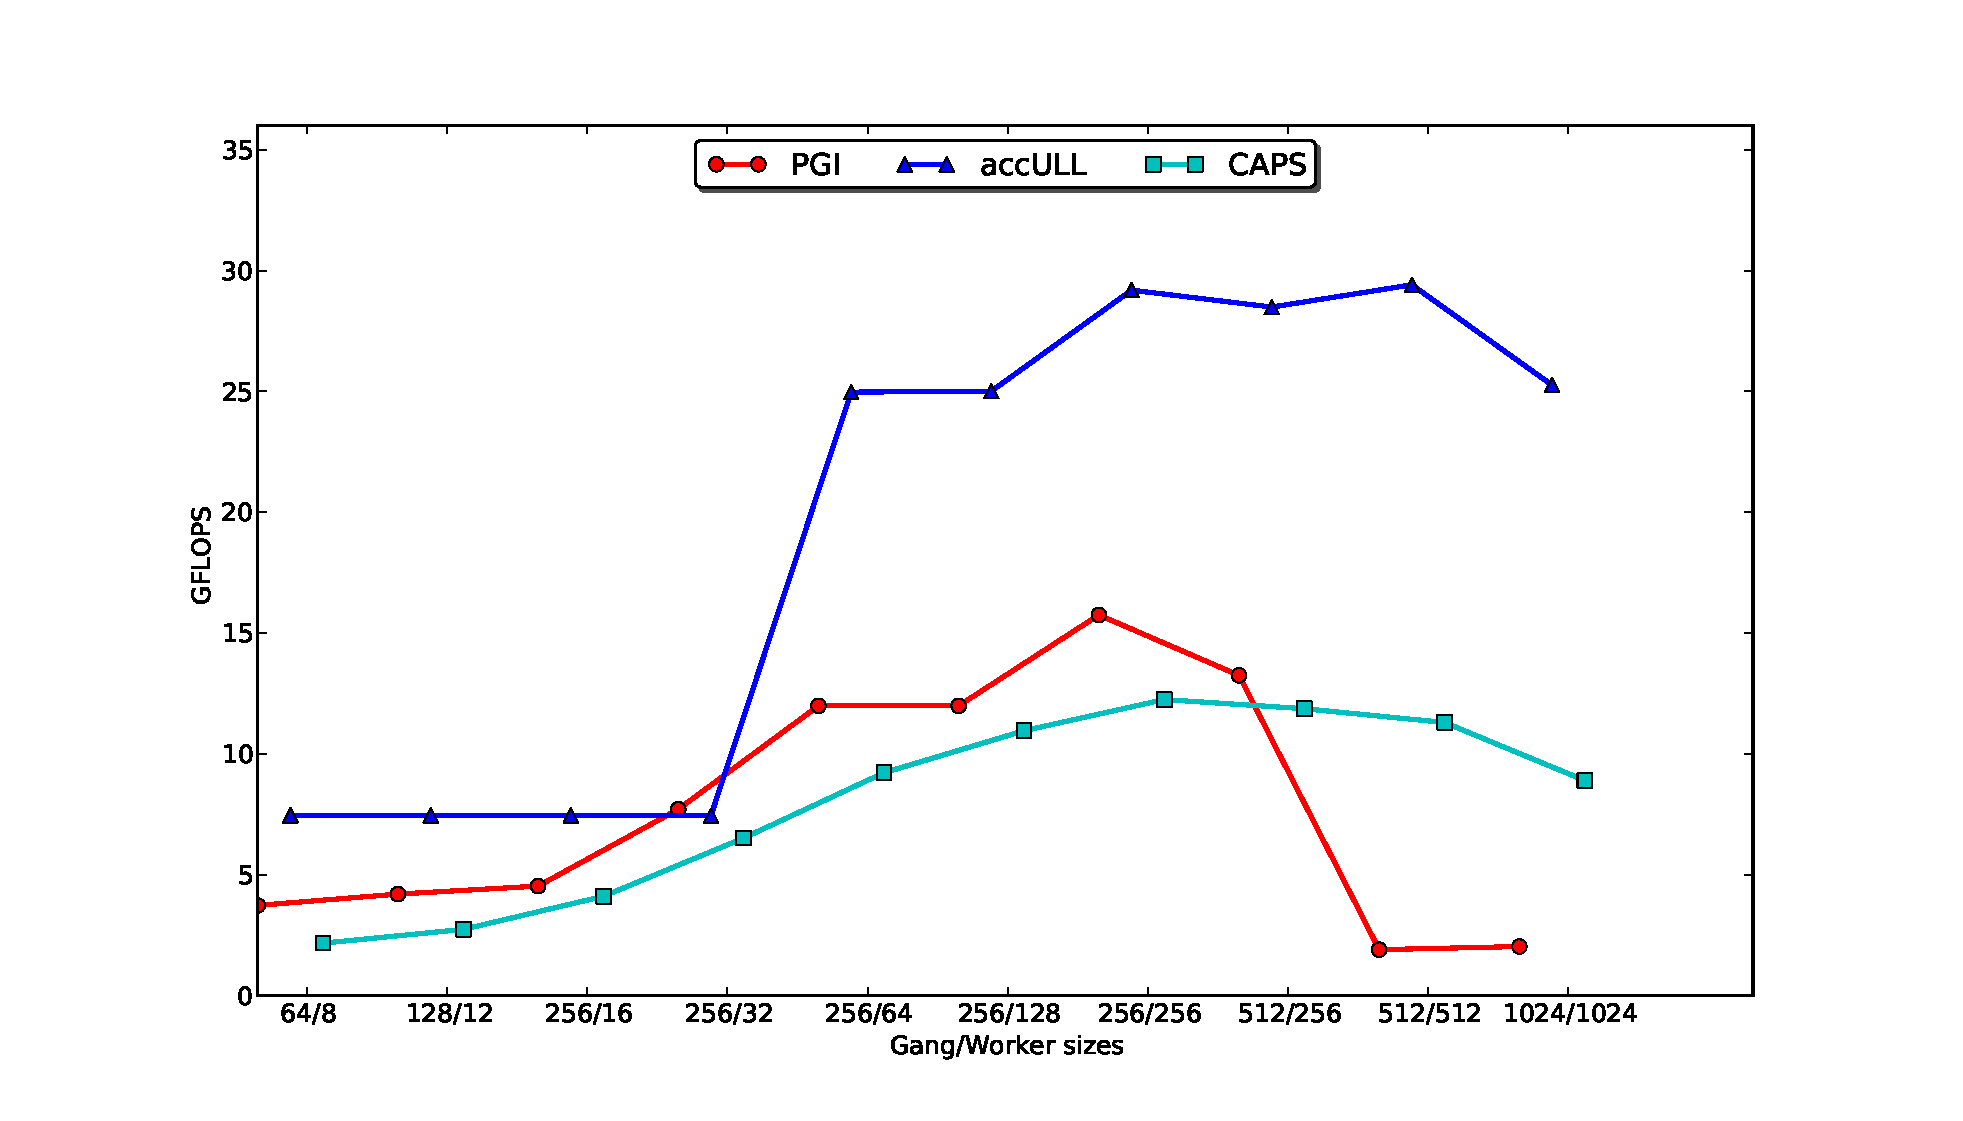
\includegraphics[width=\linewidth]{FIGURES/gemm_flops_varying}
   \caption{Rendimiento de un código \ac{MxM} con distintos valores para un mismo entorno de ejecución.}
   \label{fig:gemm_gangworker}
\end{figure}
%%%%%%%%%%%%%%%%%%%%%%%%%%%%%%%%%%%%%%%%%%%%%%%%%%%%%%%%%%%%%%%%%%%%%%%%%%%%%%%%%%%%%%%%%%


\section{\epcc{} \OpenACC{} \benchmark{} suite}
\label{sec:epccBS}

La suite del \epcc{} \OpenACC{} \benchmark{} \cite{URL::ACCepccB}
publicada en abril de 2013 por N. Johnson y A. Jackson, 
se compone de una serie de operaciones de bajo nivel diseñadas para
verificar el rendimiento potencial de los compiladores y el hardware, además de  
un conjunto de operaciones críticas que simulan aquellas encontradas en los códigos
científicos más frecuentes. 
Esta \textit{suite} está diseñada para ser usada tanto por programadores de aplicaciones 
como por aquellos administradores de sistemas que deseen medir el rendimiento de distintas 
aplicaciones en sus propios equipos informáticos. Usando para ello sus compiladores
y así poder evaluarlos frente a otros sistemas.

La suite la componen 5046 líneas de código de las cuales 140 líneas se corresponden a
etiquetas del tipo \texttt{\#pragma}. Está dividida en varios niveles de complejidad 
creciente. Un primer nivel \textit{level0} formado por códigos simples que verifican 
el correcto funcionamiento de cláusulas como \texttt{copyin}, \texttt{copyout}, etc. y 
pequeñas regiones 
de tipo \texttt{parallel} y \texttt{kernels} con bucles 1D. El segundo nivel, algo más
complejo, contiene códigos con regiones de bucles 2D, reducciones simples, así como
reducciones en kernels 2D. Por último, la suite de \benchmark{}s del \epcc{} se completa 
con el nivel 2, formado por tres códigos de aplicaciones reales habituales en 
diferentes disciplinas científicas.

%%%%%%%%%%%%%%%%%%%% Code  %%%%%%%%%%%%%%%%%%%%%%%%%%%%%%%%%%%
\begin{lstlisting}[caption={Test ATAX del level1},label=code:epcc:atax]
#pragma acc data copyin(A[0:n*n], x[0:n]), create(tmp[0:n])
{
#pragma acc parallel loop private(tmpscalar)
    for (i = 0; i < n; i++){
      tmpscalar = 0;
#pragma acc loop reduction(+:tmpscalar)
      for (j = 0; j < n; j++){
        tmpscalar += A[i*n+j] * x[j];
      }
      tmp[i] = tmpscalar;
    }
    ...
}
\end{lstlisting}
%%%%%%%%%%%%%%%%%%%%%%%%%%%%%%%%%%%%%%%%%%%%%%%%%%%%%%%%%%%%%%

Es importante destacar las reducciones en kernels 2D como 
la mostrada en el Listado \ref{code:epcc:atax} correspondiente al test ATAX. 
El test ATAX, como algunos 
otros del \textit{level1} alberga una región \texttt{parallel} 2D en la que al segundo 
bucle se le aplica una reducción (línea 6) de una variable que es privada al primer bucle 
(línea 3). Esta es una región para la que no es posible distribuir completamente el 
espacio de iteraciones en dos dimensiones como se explicó en la Sección 
\ref{subsec:ecuations}. Esto se debe a que no es posible garantizar la sincronización
entre bloques de \thread{}s, y por lo tanto la variable privada de reducción no asignará
correctamente el resultado real al vector \texttt{tmp}. Como solución provisional,
en \accULL{} se ha optado por evitar distribuir las iteraciones del segundo bucle, 
ejecutando secuencialmente sus iteraciones en cada \thread{} de \gpu{}. La versión 
evaluada de \CAPS{} no es 
capaz de compilar y ejecutar correctamente este tipo de códigos. Se tomará para la 
comparativa la versión de \PGI{} que sí que lo logra.


%%%%%%%%%%%%%%%%%%%%% Table %%%%%%%%%%%%%%%%%%%%%%%%%%%%%%%%%
\begin{table}[htb]
\caption{Tiempos de compilación de los ficheros que componen el \benchmark{}}
\label{table:epccBS:compilation}
\newcommand{\m}{\hphantom{$-$}}
%\newcommand{\cc}[1]{\multicolumn{1}{c}{#1}}
\renewcommand{\tabcolsep}{4pt} % enlarge column spacing
\renewcommand{\arraystretch}{1.2} % enlarge line spacing
\centering
\begin{tabular}{@{}ccccccc}
\hline 
       & Fichero  & Nº de Líneas & Nº de Pragmas &  PGI & CAPS HMPP    & \accULL{} \\ \hline
%\multirow{1}{*}{HS}  
      &  common.c    & 218 & 2 &  0m 0.41s  &  0m24.362s  &  0m 7.21s   \\ \hline
      &  main.c      & 189 & 2 &  0m 3.39s  &  0m32.869s  &  0m 23.612s  \\ \hline
      &  level0.c    & 767 & 45 &  1m 9.67s  &  3m47.581s  &  7m 18.67s  \\ \hline
      &  level1.c    & 1507 & 70 &  1m 22.50s &  2m50.224s  &  20m 48.98s \\ \hline
      &  27stencil.c & 246 & 8 &  0m 6.44s  &  0m42.000s  &  0m 59.05s  \\ \hline
      &  le\_core.c   & 906 & 6 &  0m 7.89s  &  0m44.579s  &  6m 16.00s  \\ \hline
      &  himeno.c    & 279 & 4 &  0m 6.48s  &  0m43.460s  &  0m 51.75s  \\ \hline
      &  Total        & 4112 & 137 &  2m 54.57s &  9m51.493s  &  36m 46.43s \\ \hline
\end{tabular}\\[2pt]
\end{table}
%%%%%%%%%%%%%%%%%%%%%%%%%%%%%%%%%%%%%%%%%%%%%%%%%%%%%%%%%%%%%%

La Tabla \ref{table:epccBS:compilation} muestra el tiempo de compilación de la suite,
con los compiladores evaluados. Destaca el buen rendimiento del compilador de \PGI{}.
En el caso de \accULL{}, su relativa falta de velocidad en el tiempo de compilación
de algunos códigos, es debida en parte a una creciente \acf{TS} que gestiona los símbolos
mediante listas. Haciendo que la búsqueda en la misma sea ineficiente. 
Entre los trabajos futuros se encuentra mejorar la \ac{TS} permitiendo una búsqueda 
mediante funciones de dispersión.
%, también conocidas como funciones \textit{hash}. 
Otro aspecto a evitar con el fin de mejorar los tiempos de compilación, es la
reiterada sucesión de ciclos de parseo y volcado del AST a código fuente, en concreto
en la clase \class{Outliner} de la que hacen uso los diferentes mutadores del \backend{}
de \package{Frangollo}.


%%%%%%%%%%%%%%%%%%%%%%%%%%%%%%%%%%%%% Figure %%%%%%%%%%%%%%%%%%%%%%%%%%%%%%%%%%%%%%%%%%%%%
\begin{figure}[!tbh]
   \centering
   \includegraphics[width=\linewidth]{resultados/epcc_acel_l0}
   \caption{Comparativa de \benchmark{}s del \textit{level0} respecto a \PGI{}}
   \label{fig:epcc_acel_level0}
\end{figure}
%%%%%%%%%%%%%%%%%%%%%%%%%%%%%%%%%%%%%%%%%%%%%%%%%%%%%%%%%%%%%%%%%%%%%%%%%%%%%%%%%%%%%%%%%%

En los tests evaluados se ha tomado un tamaño de problema 1048576.
En las Figuras \ref{fig:epcc_acel_level0}, \ref{fig:epcc_acel_level1} y 
\ref{fig:epcc_acel_level2} se puede apreciar una comparativa de los 
compiladores evaluados en la 
que se mide la aceleración respecto a \PGI{} para algunos tests destacables del 
\textit{level0}, \textit{level1} y aquellos correspondientes al nivel 2. 
A continuación se describen algunos tests que se han mostrado significativos para la 
comparativa de rendimientos entre los compiladores evaluados. 
% VALORES NEGATIVOS: VER los TEST. Por ejemplo en las reducciones indican que las reductions tandan más que el bucle sin etiquetar la reducción ( con el consiguiente resultado incorrecto)
%Para otros tests, por la naturaleza de los códigos que en muchos casos omiten devolver 
%datos, se sospecha que los compiladores han evitado descargar la región o simplemente han 
%descartado ejecutar el código en el dispositivo. 

\subsection{Nivel 0}
\label{subsec:level0}

Los cuatro primeros test miden el tiempo dedicado a las transferencias
de variables hacia y desde el dispositivo. 
Aquí \accULL{} destaca sobre el resto. 
En los test \textit{Kernels\_If} y \textit{Parallel\_If} se mide el \textit{overhead} que 
se agrega a una 
región \texttt{kernels} o \texttt{parallel}, respectivamente, que ha sido etiquetada con 
la cláusula \texttt{if(0)} para su ejecución en CPU. 
En este caso, con la región \texttt{kernels} los tiempos de \CAPS{} y 
\accULL{} son despreciables respecto a \PGI{}. 
Con la región \texttt{parallel},
\accULL{} da un resultado inferior respecto a \PGI{}. Esto se debe a que el registro 
de variables que han de ser transferidas se realiza independientemente de si se va 
ejecutar un kernel en CPU o en el dispositivo.
El test \textit{Update\_Host} mide el tiempo empleado en actualizar una variable en CPU 
después de ser asignada en \GPU{} mediante una región \texttt{kernels}, repetida después 
de la actualización.
En este test, \accULL{} tiene un comportamiento similar a \CAPS{}. \PGI{} podría estar 
omitiendo la ejecución del segundo kernel al realizar un análisis ulterior.
En el test \textit{Kernels\_Invocation} se mide el tiempo correspondiente a 
la invocación de los kernels.
Aquí, el análisis de variables que realiza \accULL{} y la forma en que el test trata de 
medir la invocación puede estar dando mejores resultados para \PGI{}. % <- CONFIRMAR !
% Se mide el tiempo de la ejecución de dos kernels por separado que han de ser ejecutados 
% en serie, al % depender el uno del otro, y posteriormente se substrae el tiempo de 
% ejecución de un kernel combinado. % O eso entiendo. Si es así habría que revisarlo
El último test evaluado, el test \textit{Parallel\_Invocation}, trata de medir la 
invocación de las 
regiones \texttt{parallel} siguiendo el mismo principio descrito para el test 
\textit{Kernels\_Invocation}. En ambos casos los resultados son similares.
% Si el anterior está mal este también !! Parece un copia y pega. % CONFIRMAR !

\subsection{Nivel 1}

%%%%%%%%%%%%%%%%%%%%%%%%%%%%%%%%%%%%% Figure %%%%%%%%%%%%%%%%%%%%%%%%%%%%%%%%%%%%%%%%%%%%%
\begin{figure}[h]
   \centering
   \includegraphics[width=\linewidth]{resultados/epcc_acel_l1}
   \caption{Comparativa de \benchmark{}s del \textit{level1} respecto a \PGI{}}
   \label{fig:epcc_acel_level1}
\end{figure}
%%%%%%%%%%%%%%%%%%%%%%%%%%%%%%%%%%%%%%%%%%%%%%%%%%%%%%%%%%%%%%%%%%%%%%%%%%%%%%%%%%%%%%%%%%

En la Figura \ref{fig:epcc_acel_level1} se presentan algunos resultados de la comparativa
del \textit{level1}. \accULL{} destaca en el test \textit{2MM}, que etiqueta una región 
\texttt{parallel} con tres bucles aplicando una reducción privada al tercero. En la 
práctica
se trata de un código similar al estudiado en el Listado \ref{code:mxm:opt1} puesto que
reduce las operaciones del tercer bucle en una variable privada que en \GPU{} se gestiona
mediante registros.
El test \textit{3MM}, similar a \textit{2MM}, emplea regiones \texttt{parallel} con 
accesos a memoria 
global, para las que \accULL{}-0.3alpha aún no aplica las optimizaciones explicadas en el 
Listado \ref{code:mxm:opt1}. % CONFIRMAR !
Se espera que cuando esta optimización se aplique se obtenga un resultado similar al
obtenido con el test \textit{2MM}.
Los tests \textit{ATAX}, \textit{BICG}, \textit{MVT}, y \textit{GESUMMV} se presentan con 
regiones \texttt{parallel} 2D con 
reducciones privadas en el segundo bucle, del tipo mostrado en el Listado 
\ref{code:epcc:atax}. Como se comentó al inicio de la presente Sección \ref{sec:epccBS},
este es un caso para el que \accULL{} aún puede aplicar algunas mejoras. Cabe destacar que 
con la versión evaluada del compilador de \CAPS{}, estos tests no se han podido compilar. 
Los tests \textit{SYRK} y \textit{COV}, que implementan regiones \texttt{parallel} 2D se 
comportan bien con \accULL{}. El motivo es que en este test hay tantos
\thread{}s disponibles - el valor aplicado en \accULL{}-0.3alpha por defecto es de 16x16 a 
cada bucle - suficientes como para que las ecuaciones de distribución de bucles (véase 
Sección \ref{subsec:ecuations}) hagan su trabajo para las $N^2 = 1048576^2$ iteraciones. 
Esto se refleja en el buen resultado de \accULL{} respecto a \PGI{}. 
En el test \textit{GEMM} se emplea una región \texttt{kernels} 2D para la que \accULL{} 
aún no aplica las ecuaciones de distribución de iteraciones mencionadas. Por lo que queda 
margen para mejorar estos resultados. 
% XXX
%Los tests 2DCONV y 3DCONV alojan regiones \texttt{kernels 
%loop independent}, y sus resultados aún han de ser estudiados. % CONFIRMAR !

%%%%%%%%%%%%%%%%%%%%%%%%%%%%%%%%%%%%% Figure %%%%%%%%%%%%%%%%%%%%%%%%%%%%%%%%%%%%%%%%%%%%%
\begin{figure}[!tbh]
   \centering
   \includegraphics[width=0.9\linewidth]{resultados/epcc_acel_l2}
   \caption{Comparativa de \benchmark{}s del \textit{level2} respecto a \PGI{}}
   \label{fig:epcc_acel_level2}
\end{figure}
%%%%%%%%%%%%%%%%%%%%%%%%%%%%%%%%%%%%%%%%%%%%%%%%%%%%%%%%%%%%%%%%%%%%%%%%%%%%%%%%%%%%%%%%%%

\subsection{Nivel 2}
En la Figura \ref{fig:epcc_acel_level2} se muestran los resultados de la ejecución
respecto al tiempo de \PGI{} con los compiladores evaluados. Estos son tests 
basados en programas científicos reales con una complejidad considerable.
El núcleo pesado de 27S está compuesto de dos regiones \texttt{parallel} 3D, que
\accULL{} convierte en kernels 2D con la consiguiente pérdida de rendimiento.
LE2D contiene dos regiones 2D, que son una región \texttt{kernels} y otra 
\texttt{parallel}. Ambas etiquetadas con cláusulas \texttt{present} que \accULL{} 
gestiona mediante ámbitos adecuadamente. 
LE2D repite la llamada a estas regiones de manera reiterada. Repitiendo el proceso
400 veces. Se estima que el bajo rendimiento en \accULL{} se debe a el \textit{overhead}
de la invocación de las regiones, tal como se pudo apreciar en la Sección 
\ref{subsec:level0} con los tests \textit{Kernels\_Invocation} y \textit{Parallel\_Invocation}. % CONFIRMAR!

En muchos casos las regiones \texttt{parallel} pueden estar distribuyendo las iteraciones 
en una pequeña cantidad de \thread{}s - en \accULL{}-0.3alpha si no se indica nada mediante 
las cláusulas \gang{} y \worker{} por defecto se asignan 16 bloques de 16 \thread{}s cada 
uno. Pese al bajo rendimiento de algunos de estos resultados, el mayor logro estriba en 
lograr que \accULL{} compile y ejecute una serie de códigos escritos en \OpenACC{} por un 
tercero autorizado, en este caso investigadores miembros del \epcc{}. Como línea de 
trabajo futuro se tratará de analizar y estudiar cómo mejorar el rendimiento de estos 
códigos, que sin duda alguna han servido para evaluar cualitativamente el framework
de compilación que compone \accULL{}.

%%
% ---------------------------------------------------
%
% Proyecto de Final de Carrera:
% Author: José Lucas Grillo Lorenzo <jlucas.gl@gmail.com>
% Capítulo: Conclusiones y trabajos futuros
% Fichero: Cap7_conclusiones.tex
%
% ----------------------------------------------------
%


\chapter{Conclusiones y trabajos futuros} \label{chap:conclusiones}  

\section{Conclusiones} \label{sec:conclusiones}

En el presente \acf{PFC}, se han abordado los asuntos relativos a las 
optimizaciones de bucles y su implementación, mediante las cláusulas \gang{} y \worker{}, 
en el contexto del estándar de programación heterogénea basado en directivas \OpenACC{}. 
No menos importante ha sido todo el trabajo de depuración y optmización del código que
compone el compilador, para obtener una versión de \accULL{} capaz de compilar 
satisfactoriamente los códigos evaluados. Así mismo es destacable también el trabajo
realizado por el autor para lograr elaborar un producto listo para usar a partir del
software del que está compuesto \accULL{}. 
Importante ha sido en esta labor el trabajo con las
herramientas de versionado y gestión de repositorio, sin las cuales las tareas de 
depuración y publicación de \textit{release} hubieran sido mucho más tediosas.
%XXX - Pasa revista a lo que has hecho:
En esta memoria de PFC se han revisado los logros conseguidos en la ejecución del 
proyecto. Relacionándolos directamente con los objetivos planteados inicialmente, podemos 
señalar como más significativos los siguientes logros: 
%(pon los más directos, los menos abstractos)

Se ha conseguido que \accULL{} compile y genere código correcto, 
comprobándolo en tiempo de ejecución para los niveles 0 y 1 del benchmark del EPCC 
\cite{URL::ACCepccB}, así como para los códigos \textit{27stencil} y \textit{le\_core} del 
nivel 2. Previo a la realización de este \ac{PFC} solo era posible compilar el nivel 0 y 
algunos códigos sencillos del 
nivel 1. El test \textit{le\_core} tampoco compilaba debido a diversos problemas con la 
\ac{TS}. Concretamente, no había soporte para la definición encadenada de tipos mediante 
\texttt{typedef}, y las opciones disponibles entonces estaban muy limitadas y daban serios 
problemas al volver a parsear el código, una vez volcado.

El grado de madurez alcanzado por \accULL{} es tal que a través de los experimentos 
realizados (véase Capítulo \ref{chap:resultados}) \accULL{} se ha convertido en una 
herramienta suficientemente madura para ofrecer resultados comparables en muchos casos a los 
que se pueden conseguir con herramientas comerciales.
No se pretende con ello decir que \accULL{} sea una herramienta acabada. En muchos casos 
somos conscientes de sus limitaciones; pueden aparecer bugs, el tiempo de compilación es 
en muchos casos elevado, el manejo de errores es mejorable, etc.
Entre estas limitaciones destaca el compilador (\yacf{}). Un compilador escrito en Python, 
un lenguaje interpretado, que tiene algunas carencias. Entre ellas una búsqueda en la 
Tabla de Símbolos ineficiente, o el hecho repetir varios ciclos de parseo y volcado de 
código en sucesivas etapas, hacen que \yacf{} sea uno de los puntos débiles de \accULL{}. 
En este sentido los ciclos de parseo-volcado nos han permitido desarrollar optimizaciones 
y transformaciones de código con relativa facilidad. No obstante es 
evidente la necesidad de estudiar sustituir el actual compilador \yacf{} basado en 
\textit{pycparser} \cite{Bendersky:pyc:2009}
por algún otro basado en herramientas con mayor soporte.

\section{Trabajos futuros} \label{sect:trabajo}

%Clasifícalos como 'cosas que vamos a acometer en breve' y 'cosas de mucha enjundia'.
Se clasifican a continuación, en orden de más prioritario a menos, las líneas abiertas de 
trabajos futuros que han de ser acometidos próximamente en el contexto de la 
investigación con el framework de compilación \accULL{}.

\begin{itemize}
\item Solucionar los casos de resultados incorrectos cuando haya que distribuir menos 
iteraciones que los \thread{}s de los que se disponga, al aplicar la planificación 
mediante las cláusulas \texttt{num\_gangs} y \texttt{num\_workers}, o en general al 
invocar a las cláusulas \gang{}/\worker{}.
\item Dar soporte para las reducciones de variables privadas en kernels de 2 o más 
dimensiones.
\item Evaluar la plataforma con más \benchmark{}s siguiendo el trabajo llevado a cabo para 
fortalecer su robustez. Como trabajo inmediato, está previsto evaluar los \textit{NAS 
Parallel \benchmark{}} \cite{Bailey:1991:NPB} verificando la correcta ejecución de los 
experimentos, y depurando a su vez los hipotéticos \textit{bugs} que surjan.
\item Implementar el soporte para las cláusulas \gang{}/\worker{} en regiones de tipo 
\texttt{kernels}, ya que actualmente solo están disponibles para regiones 
\texttt{parallel}.
\item Experimentar de forma intensiva con aplicaciones reales. Aprovechando las 
colaboraciones con el grupo del Dr. D. C. García Sanchez de la Universidad Complutense de 
Madrid, así como con 
el \ac{IAC} - a través del profesor Dr. D. F. Garzón, y el Dr. D. Antonio Dorta - este 
último miembro del grupo de 
investigación \GCAP{}.
\item Dar soporte para kernels 3D. 
\item Reemplazar \yacf{} por alguna alternativa más robusta como podría ser Cetus 
\cite{Lee:2003:CEC}, 
Rose \cite{Liao:2010:ESS}, Mercurium \cite{URL::Mercurium}, o LLVM \cite{Guntli:2011:AC}, 
como se ha discutido en la Sección \ref{sec:conclusiones}.
\end{itemize}
 
 %
% ---------------------------------------------------
%
% Proyecto de Final de Carrera:
% Author: José Lucas Grillo Lorenzo <jlucas.gl@gmail.com>
% Capítulo: To Do 
% Fichero: Cap_todo.tex
%
% ----------------------------------------------------
%

% Notas:
% 	Evitar coloquialidad
% 	Evitar cuantificadores gratuitos: un poco, muy caro, ...
% 	UNIFORMIDAD
% 	Completitud
% 	Hemos hecho, se ha desarrollado, 
% 	La siguiente Figura NO: la Figura XXX. El Listado XXX.
% 	Cada vez que hagas una afirmación "rotunda", AVÁLALA

\chapter{To Do} \label{chap:to-do} 

\section{Pendiente}

\begin{itemize}
\item Para rodinia pon las referencias (a Rodinia) que aparecen en los últimos Papers. https://www.cs.virginia.edu/~skadron/wiki/rodinia/index.php/Main\_Page
\item -----------------------------------------------------------------
\item Escribir los agradecimientos
\item Terminar y revisar el Capítulo Resultados computacionales (Capítulo 6)
\item Presentación
\item Enviar memoria
\end{itemize}

\section{Hecho}
\begin{itemize}
\item Definir un primer esqueleto de la memoria
\item Añadido Capítulo \ref{chap:optGPGPU}: Optimizaciones en GPGPU
\item Trabajando con texmaker y corrector ortográfico
\item Traducir y resumir el Capítulo de \yacf{} (Capítulo \ref{chap:yacf})
\item Introducción al Capítulo sobre el modelo poliédrico (Capítulo 2)
\item Revisado y adaptado el Prólogo
\item Primer esqueleto del Capítulo de Resultados.
\item En el cap. de Resultados: Introd. a Rodinia, qué es, referencias, características de los códigos para los que presentas resultados
\item Descripción de la plataforma de desarrollo (Verode)
\item Escribir el Capítulo de Motivaciones (Capítulo \ref{chap:motivation})
\item Escribir Optimizaciones en GPGPU (Capítulo \ref{chap:optGPGPU})
\item Escribir objetivos del \ac{PFC} (Capítulo \ref{chap:objetives})
\item Revisar y mejorar el prólogo
\item -----------------------------------------------------------------
\item También en resultados: Añadir referencia al benchmark del EPCC (URL)
\item Descripción de software (versiones de 3 compiladores)
\item -----------------------------------------------------------------
\item Añadir las referencias al documento
\item Añadir a las motivaciones el ``Trabajo relacionado''
\item Añadir al Prólogo, el esquema de la memoria los Capítulos que contiene
\end{itemize}

\section{Revisión final}
\begin{itemize}
%\item Aspell
\item Comprobar los Listados
\item Comprobar referencias perdidas y XXX 
\end{itemize}


% ==========================================================
% ----------              Apendices                ---------
% ----------   Estan en el directorio apendices/   ---------
% ==========================================================
% \appendix
% \cleardoublepage
% \addappheadtotoc
% \appendixpage
% % Apéndices
% %
% ---------------------------------------------------
%
% Proyecto de Final de Carrera:
% Author: José Lucas Grillo Lorenzo <jlucas.gl@gmail.com>
% Apéndice: A1
% Fichero: Ap1_XXX.tex
%
% ----------------------------------------------------

\chapter{Códigos relacionados} 
\label{ap:apx_1}

A continuación se presentan 1770 líneas de código repartidas en varios ficheros
pertenecientes al trabajo realizado respecto a las optimizaciones de bucles,
aunque hay que aclarar que los desarrollos llevados a cabo no se limitan a
los códigos aquí presentados. Estos son códigos que han sido aportados y
desarrollados enteramente por el autor para el proyecto de investigación \accULL{}:

\section{Loop Common}
\lstinputlisting[language=Python,caption={Módulo \package{Common.py} conteniendo
filtros y mutadores útiles para las optimizaciones}, label={code:common.py}]
{listings/Common.py} %% LISTING

\section{Loop interchange}
\lstinputlisting[language=Python,caption={Módulo \package{LoopInterchange.py}
que alberga el mutador \class{LoopInterchangeMutator}}, 
label={code:loopInterchange.py}]{listings/LoopInterchange.py} %% LISTING

\section{Loop StripMining}
\lstinputlisting[language=Python,caption={Módulo \package{LoopStripMining.py}
que alberga el mutador \class{LoopStripMiningMutator}}, 
label={code:loopStripMining.py}]
{listings/LoopStripMining.py} %% LISTING

\section{Loop Tiling}
\lstinputlisting[language=Python,caption={Módulo \package{LoopTiling.py}
que alberga el mutador \class{LoopTilingMutator}}, 
label={code:loopTiling.py}]
{listings/LoopTiling.py} %% LISTING

\section{Driver accgangworker.py}
\lstinputlisting[language=Python,caption={Driver \package{accgangworker.py}
descrito en la Sección \ref{chap:optGPGPU:accgangworker}}, 
label={code:accgangworker.py}]
{listings/accgangworker.py} %% LISTING


\section{Acc Parallel Loop}
\lstinputlisting[language=Python,caption={Clase \class{AccParallelLoopMutator}
encargada de realizar las transformaciones correspondientes a las cláusulas
\gang{} y \worker{}}, 
label={code:accparallelloop}]
{listings/AccParallelLoop.full.py} %% LISTING

% ==========================================================
% ---------          Bibliografia               ------------
% --------- Estan en el directorio bibliografia/------------
% ==========================================================
\backmatter
%\pagestyle{fancy}
% ELEGIR un estilo que te guste de bibliografía
%\bibliographystyle{amsplain}
%\bibliographystyle{abbrv}         % 
\bibliographystyle{bmc_article}    % Este estilo mete las URLs de la bibliografía entre brackets
% 
% Diferentes ejemplos de estilos para bibliografía:
% http://amath.colorado.edu/documentation/LaTeX/reference/faq/bibstyles.html
%
\renewcommand{\bibname}{Bibliografía}   %  Para que no aparezca Índice de figuras
\addcontentsline{toc}{chapter}{\bibname}  % Lo añade al inidice
%\markboth{\bibname}{\bibname}
\bibliography{bibliografia/bibliografia}

% ==========================================================
% ---------                Índices              ------------
% ==========================================================

\renewcommand{\listfigurename}{Índice de Figuras}   %  Para que no aparezca Índice de figuras
\addcontentsline{toc}{chapter}{\listfigurename}  % Para incluirlo en el índice  
%\markboth{\listfigurename}{\listfigurename}
\listoffigures

\renewcommand{\listtablename}{Índice de Tablas}   %  Para que no aparezca Índice de cuadros
\addcontentsline{toc}{chapter}{\listtablename}  % Para incluirlo en el índice  
%\markboth{\listtablename}{\listtablename}
\listoftables

\renewcommand{\lstlistlistingname}{Índice de Listados} %  Para que no aparezca Listings
\addcontentsline{toc}{chapter}{\lstlistlistingname}     % Para incluirlo en el índice     
%\markboth{\lstlistlistingname}{\lstlistlistingname}
\lstlistoflistings

\end{document}
